% The document will be printed one side in A4 paper.
%\documentclass[12pt,a4paper,oneside]{report}
%\documentclass[12pt,a4paper,twoside]{report}
\documentclass[12pt,a4paper,twoside]{article}

\usepackage[round]{natbib}

\usepackage[pdftex]{color,graphicx}
\usepackage{setspace}
\usepackage{a4wide}

\usepackage[a4paper]{geometry}
\usepackage[cm]{fullpage}


%subfigures deprecated
%\usepackage{subfigure}
%use subcaption instead
\usepackage{caption}
\usepackage{subcaption}
%side caption: SCfigure
%\usepackage{sidecap}
% Use PDF output.
% The output should be wide.
\usepackage{url}
%for definition list
\usepackage{enumitem}
%for celsius
%\usepackage{gensymb}
%for listing code
\usepackage{listings}
%for table cell with diagonal division
\usepackage{slashbox}
\usepackage{tabularx}
\usepackage{amsmath}

%\usepackage[graphics,tightpage,active]{preview}
%\PreviewEnvironment{tikzpicture}
%\PreviewEnvironment{equation}
%\PreviewEnvironment{equation*}
%\newlength{\imagewidth}
%\newlength{\imagescale}
%\pagestyle{empty}
%\thispagestyle{empty}
%\usepackage{standalone}

\usepackage[french, greek, english]{babel}
%input encoding
%\usepackage[iso-8859-7]{inputenc}
%\usepackage[latin1]{inputenc}
%output encoding
\usepackage[T1]{fontenc}
\selectlanguage{english}

% Pour la dedicace
\usepackage{frcursive}

\usepackage[table]{xcolor}
\usepackage{booktabs}
\usepackage{tabu}

\usepackage[section,subsection,subsubsection]{extraplaceins}
\usepackage{url} %tablerules
\usepackage{xr}
\externaldocument{supplementary}

\usepackage[labelfont=bf,labelsep=period,justification=raggedright]{caption}
\usepackage{authblk}


\setcounter{secnumdepth}{0}



%\doublespacing

%\title{Leveraging qPCR with SNP data achieves large scale case-control analysis of KIR3DL1/3DS1 copy number variation in type 1 diabetes}
\title{Predicting \emph{KIR3DL1/S1} copy number from ImmunoChip signals in large scale type 1 diabetes association study}
%and reveals no association in type 1 diabetes}
\author[1]{Nikolas Pontikos}
\author[1]{Deborah Smyth}
\author[1]{Helen Schuilenburg}
\author[1]{Joanna MM Howson}
\author[1]{Neil M. Walker}
\author[2]{Jyothi Jayaraman}
\author[2]{Wei Jiang}
\author[2]{James Traherne}
\author[2]{John Trowsdale}
\author[1]{John A. Todd}
\author[1]{Chris Wallace}
\affil[1]{JDRF/Wellcome Trust Diabetes and Inflammation Laboratory, Cambridge Institute for Medical Research, University of Cambridge, Wellcome Trust/MRC Building, Cambridge CB2 0XY, United Kingdom;}
\affil[2]{Division of Immunology, Department of Pathology, University of Cambridge, Cambridge CB2 1QP, United Kingdom}

\renewcommand\Authands{ and }


\date{}


\begin{document}

\newlength{\oparindent}
\setlength{\oparindent}{\parindent}
\setlength{\parindent}{0pt}

\maketitle
\noindent


%\newpage
%\thispagestyle{empty} 
%\addtocounter{page}{-1}
%\vspace*{\fill}
%\begin{center}
%{\fontfamily{frc}\selectfont \foreignlanguage{french} {Pour ma petite Maman ch\'erie, \`a qui je dois tout \ldots}}
%{\fontfamily{frc}\selectfont Pour ma petite Maman cherie, a qui je dois tout \ldots}
%\end{center}
%\vspace*{\fill}
%\clearpage

\abstract{
Killer Immunoglobulin-like Receptors (KIR) are important surface receptors of Natural Killer cells.
KIRs mediate the fate of target cells based on the composite inhibiting/activating signal generated on binding to their corresponding HLA (Human Leukocyte Antigen) class I ligands.
Type 1 diabetes (T1D) is an autoimmune disease strongly associated with genetic variation in the HLA region, primarily with Class II genes, but also with HLA Class I loci including HLA-Bw4, an epitope grouping both HLA-A and HLA-B alleles into HLA-Bw4-80I and HLA-Bw4-80T subgroups.
Amongst the 17 known genes of the KIR region, characterised by alternative haplotypes of variable gene copy numbers, \emph{KIR3DL1} is the only one proven to bind in-vitro with both HLA-Bw4 epitopes.
Its activating counterpart, \emph{KIR3DS1}, putatively binds the HLA-Bw4-80I epitope only.
\emph{KIR3DL1/S1} is therefore an interesting T1D candidate gene but since the KIR region is poorly characterised, genotyping with conventional SNP arrays is unreliable.
So far, insufficiently powered PCR-based genotyping studies of less than 600 individuals, have failed to detect convincing association of T1D with presence or absence of \emph{KIR3DL1/S1}.  
For the first time, we are able to test for association in a sample size of 6,744 cases and 5,362 controls, twenty-fold larger than any previous study, by using \emph{KIR3DL1/S1} copy number calls from a recently developed KIR qPCR assay in order to impute copy number in samples assayed only with ImmunoChip,
a custom Illumina genotyping chip with probes for 30 SNPs in the target region.
%with dense coverage of autoimmune regions

%The \emph{KIR3DL1/S1} copy numbers from qPCR data were called by clustering jointly on the $\Delta$Ct values of \emph{KIR3DL1} and \emph{KIR3DS1}.
%The imputed \emph{KIR3DL1/S1} copy numbers from SNP data were predicted from Log R Ratio and B Allele Frequency with a 1.3\% misclassification error rate
%in leave-one-out cross-validation in the \emph{KIR3DL1/S1} region using a nearest neighbour classifier trained on 747 case and 727 control samples analysed
%both with qPCR and on Immunochip, a custom SNP array.
The association of \emph{KIR3DL1/S1} copy number with T1D was tested in all samples and conditional on the corresponding HLA-Bw4 ligand subsets.
The interaction effect between \emph{KIR3DL1/S1} and HLA-Bw4 was also tested with a case-only analysis.
We can confirm from our study with a substantially increased sample size, that copy number variation in \emph{KIR3DL1/S1} is not an important modifier of T1D risk (0.9 < OR < 1.1 at 95\% confidence for the common genotype), either alone or dependent on HLA-Bw4 epitope, and that furthermore, there is no evidence of statistical interaction effect between HLA-Bw4 and \emph{KIR3DL1/S1} copy number in T1D.  
\emph{( 340 words )}
%This implies that NK are unlikely to be important players in the aetiology of T1D.
%This presents evidence against the role of NK cells in the aetiology of T1D.
%The association is not caused by the interaction with KIR
%These results suggest that HLA Class I susceptibility alleles do not mediate risk to T1D through interplay with KIR3DL1/S1 which would imply that NK cells are not causal of T1D
%These results suggest that the interplay between KIR and HLA may not be an signifcant risk factor in aetology of T1D.
%This strengthens the hypothesis that NK cells are not involved in aetiology of T1D.
}


\doublespacing
%\onehalfspacing

\section{Introduction}
%%
% A header that lets you compile a chapter by itself, or inside a larger document.
% Adapted from http://stackoverflow.com/questions/3655454/conditional-import-in-latex
%
%
%Use \inbpdocument and \outbpdocument in your individual files, in place of \begin{document} and \end{document}. In your main file, put in a \def \ismaindoc {} before including or importing anything.
%
% David Duvenaud
% June 2011
% 
% ======================================
%
%


\ifx\ismaindoc\undefined
	\newcommand{\inbpdocument}{
		\def \ismaindoc {}
		% Use this header if we are compiling by ourselves.
		\documentclass[a4paper,11pt]{common/PhDThesisPSnPDF}
		\usepackage[round]{natbib} 
\usepackage{hyperref} 
\usepackage{url} %tablerules
\usepackage{cleveref}
\usepackage{soul}


%\usepackage{draftwatermark}
%\SetWatermarkLightness{0.95}

% ******************************************************************************
% ****************************** Custom Margin *********************************

% Add `custommargin' in the document class options to use this section
% Set {innerside margin / outerside margin / topmargin / bottom margin}  and
% other page dimensions

\ifsetMargin
\else
    \RequirePackage[left=37mm,right=30mm,top=35mm,bottom=30mm]{geometry}
    \setFancyHdr % To apply fancy header after geometry package is loaded
\fi


%\chead{Unfinished draft}
\cfoot{\texttt{Unfinished draft - compiled on \today{} at \currenttime}}

% *****************************************************************************
% ******************* Fonts (like different typewriter fonts etc.)*************

% Add `customfont' in the document class option to use this section

\ifsetFont
\else
    % Set your custom font here and use `customfont' in options. Leave empty to
    % load computer modern font (default LaTeX font).  

    \RequirePackage{libertine} 
\fi



% Add appendices
\RequirePackage[title,titletoc]{appendix}

% changes the default name `Bibliography` -> `References'
%\renewcommand{\bibname}{References}


% *****************************************************************************
% *************** Changing the Visual Style of Chapter Headings ***************
% Uncomment the section below. Requires titlesec package.

%\RequirePackage{titlesec}
%\newcommand{\PreContentTitleFormat}{\titleformat{\chapter}[display]{\scshape\Large}
%{\Large\filleft{\chaptertitlename} \Huge\thechapter}
%{1ex}{}
%[\vspace{1ex}\titlerule]}
%\newcommand{\ContentTitleFormat}{\titleformat{\chapter}[display]{\scshape\huge}
%{\Large\filleft{\chaptertitlename} \Huge\thechapter}{1ex}
%{\titlerule\vspace{1ex}\filright}
%[\vspace{1ex}\titlerule]}
%\newcommand{\PostContentTitleFormat}{\PreContentTitleFormat}
%\PreContentTitleFormat


% *****************************************************************************
% **************************** Custom Packages ********************************
% *****************************************************************************


% ************************* Algorithms and Pseudocode **************************

%\usepackage{algpseudocode} 


% ********************Captions and Hyperreferencing / URL **********************

% Captions: This makes captions of figures use a boldfaced small font. 
%\RequirePackage[small,bf]{caption}

\RequirePackage[labelsep=space,tableposition=top]{caption} 
\renewcommand{\figurename}{Fig.} %to support older versions of captions.sty
\captionsetup{belowskip=12pt,aboveskip=4pt}

% ************************ Formatting / Footnote *******************************

%\usepackage[perpage]{footmisc} %Range of footnote options 


% ****************************** Line Numbers **********************************

%\RequirePackage{lineno}
%\linenumbers

% ************************** Graphics and figures *****************************

\usepackage{rotating}
\usepackage{lscape} 
%\usepackage{wrapfig}
%\usepackage{float}
%subfigures deprecated
%\usepackage{subfigure}
%use subcaption instead
\usepackage[labelfont=bf,labelsep=period,justification=raggedright]{caption}
\usepackage{subcaption}
%\usepackage{subfig} %note: subfig must be included after the `caption` package. 


% ********************************* Table **************************************

%for table cell with diagonal division
%\usepackage{multicol}
\usepackage{multirow}
\usepackage{tabularx}
\usepackage{slashbox}
\usepackage{longtable} 
\usepackage{booktabs}
\usepackage{tabu}
\usepackage{xcolor,colortbl}



% ***************************** Math and SI Units ******************************

\usepackage{amsthm}
\usepackage{amsfonts}
\usepackage{amsmath}
\usepackage{amssymb}
\usepackage{textcomp}
% degree celsius
%\usepackage{gensymb}
%percentages, microliters, nanograms etc
\usepackage{siunitx}
\DeclareSIUnit[number-unit-product={}]\unit{U}


% ******************************************************************************
% ************************* User Defined Commands ******************************
% ******************************************************************************

% *********** To change the name of Table of Contents / LOF and LOT ************

%\renewcommand{\contentsname}{My Table of Contents}
%\renewcommand{\listfigurename}{My List of Figures}
%\renewcommand{\listtablename}{My List of Tables}


% ********************** TOC depth and numbering depth *************************

%\setcounter{secnumdepth}{2}
%\setcounter{tocdepth}{2}

% ******************************* Nomenclature *********************************

% To change the name of the Nomenclature section, uncomment the following line

%\renewcommand{\nomname}{Symbols}


% ********************************* Appendix ***********************************

% The default value of both \appendixtocname and \appendixpagename is `Appendices'. These names can all be changed via: 

%\renewcommand{\appendixtocname}{List of appendices}
%\renewcommand{\appendixname}{Appndx}


%%% Packages
% Use Charter font.
%\usepackage{charter}
% for line spacing
\usepackage{setspace}
\usepackage{xspace}
% Use PDF output.
%\usepackage[pdftex]{color,graphicx}
% The output should be wide.
%\usepackage{a4wide}
%\usepackage[a4paper]{geometry}
%\usepackage[text={7.5in,9in},centering]{geometry}
%\usepackage[cm]{fullpage}
%for definition list
\usepackage{enumitem}
%puts silly zeroes in section names
%\usepackage{fancyhdr}
%for code snippets
%\usepackage{float}
%\floatstyle{ruled}
%\newfloat{program}{thp}{lop}
%\floatname{program}{Code snippet} 
\usepackage{tikz}
\usetikzlibrary{shapes,arrows,calc,through,backgrounds,decorations.pathmorphing,shadows} 
%\usepackage[active,tightpage]{preview} 
\usepackage[french, greek, english]{babel}
%input encoding
%\usepackage[iso-8859-7]{inputenc}
%\usepackage[latin1]{inputenc}
%output encoding
\usepackage[T1]{fontenc}
\selectlanguage{english} 
% Pour la dedicace
\usepackage{frcursive} 
%side caption: SCfigure
%\usepackage{sidecap}
%\usepackage[table]{xcolor}
%\usepackage[graphics,tightpage,active]{preview}
%\PreviewEnvironment{tikzpicture}
%\PreviewEnvironment{equation}
%\PreviewEnvironment{equation*}
%\newlength{\imagewidth}
%\newlength{\imagescale}
%\pagestyle{empty}
%\thispagestyle{empty}
%\usepackage{standalone} 
\usepackage[section,subsection,subsubsection]{extraplaceins} 
\usepackage{authblk} 
\usepackage{graphicx} 
%unicode support
\usepackage[utf8]{inputenc} 
%multiple indices
\usepackage{multind}
%glossary
\usepackage[acronym]{glossaries}

\usepackage{datetime}
\renewcommand{\tabularxcolumn}[1]{>{\arraybackslash}m{#1}}
\usepackage{relsize}
\usepackage{nicefrac}
\usepackage{nth}
\usepackage{array}




		% All my custom preamble stuff.  Shouldn't overlap with anything in official-preamble


% Paths to figure and table directories.
\newcommand{\symmetryfigsdir}{figures/symmetries}
\newcommand{\topologyfiguresdir}{figures/topology}
\newcommand{\infinitefiguresdir}{figures/infinite}
\newcommand{\grammarfiguresdir}{figures/grammar}
\newcommand{\introfigsdir}{figures/intro}
\newcommand{\gplvmfiguresdir}{figures/gplvm}
\newcommand{\warpedfiguresdir}{figures/warped-mixtures}
\newcommand{\deeplimitsfiguresdir}{figures/deep-limits}
\newcommand{\quadraturefigsdir}{figures/quadrature}
\newcommand{\additivefigsdir}{figures/additive}
\newcommand{\decompfigsdir}{figures/decomp}
\newcommand{\examplefigsdir}{figures/worked-example}


\usepackage{bm}  % for warped mixtures - is this necessary?
\usepackage{booktabs}
\usepackage{tabularx}
\usepackage{multirow}
\usepackage{datetime}
\renewcommand{\tabularxcolumn}[1]{>{\arraybackslash}m{#1}}
\usepackage{relsize}
\usepackage{graphicx}
\usepackage{amsmath,amssymb,textcomp}
\usepackage{nicefrac}
\usepackage{amsthm}
\usepackage{tikz}
\usetikzlibrary{arrows}
\usetikzlibrary{calc}
\usepackage{nth}
\usepackage{rotating}
\usepackage{array}
\usepackage[hyperpageref]{backref}


\def\foo{\hspace{\fill}\mbox{}\linebreak[0]\hspace*{\fill}}
\renewcommand*{\backref}[1]{}
\renewcommand*{\backrefalt}[4]{%
\ifcase #1 %
%
\or
\foo(page #2)%
\else
\foo(pages #2)%
\fi
}

\usepackage{cleveref}
\crefname{equation}{equation}{equations}


%% For submission, make all render blank.
\input{common/commenting.tex}
%\renewcommand{\LATER}[1]{}
%\renewcommand{\fLATER}[1]{}
%\renewcommand{\TBD}[1]{}
%\renewcommand{\fTBD}[1]{}
%\renewcommand{\PROBLEM}[1]{}
%\renewcommand{\fPROBLEM}[1]{}
%\renewcommand{\NA}[1]{}


% HUMBLE WORDS: shown slightly smaller when in normal text
% Thanks to Christian Steinruecken!
\input{common/humble.tex}


% TODO: Clean up duplicates
\declareHumble{ANOVA}{ANOVA}
\declareHumble{ARD}{ARD}
\declareHumble{BIC}{BIC}
\declareHumble{BMC}{BMC}
\declareHumble{bq}{BQ}
\declareHumble{CRP}{CRP}
\declareHumble{dirpro}{DP}
\declareHumble{HDMR}{HDMR}
\declareHumble{GAM}{GAM}
\declareHumble{GEM}{GEM}
\declareHumble{GMM}{GMM}
\declareHumble{gplvm}{GP-LVM}
\declareHumble{gpml}{GPML}
\declareHumble{GPML}{GPML}
\declareHumble{gprn}{GPRN}
\declareHumble{gpt}{GP}
\declareHumble{gp}{GP}
\declareHumble{HKL}{HKL}
\declareHumble{HMC}{HMC}
\declareHumble{ibp}{IBP}
\declareHumble{iGMM}{iGMM}
\declareHumble{iwmm}{iWMM}
\declareHumble{kCP}{CP}
\declareHumble{kCW}{CW}
\declareHumble{kC}{C}
\declareHumble{KDE}{KDE}
\declareHumble{kLin}{Lin}
\declareHumble{KPCA}{KPCA}
\declareHumble{kPer}{Per}
\declareHumble{kRQ}{RQ}
\declareHumble{kSE}{SE}
\declareHumble{kWN}{WN}
\declareHumble{Lin}{Lin}
\declareHumble{LBFGS}{L-BFGS}
\declareHumble{mcmc}{MCMC}
\declareHumble{MKL}{MKL}
\declareHumble{MLP}{MLP}
\declareHumble{MSE}{MSE}
\declareHumble{Per}{Per}
\declareHumble{RMSE}{RMSE}
\declareHumble{RQ}{RQ}
\declareHumble{SBQ}{SBQ}
\declareHumble{seard}{SE-ARD}
\declareHumble{sefull}{SE-\textnormal{full}}
\declareHumble{SEGP}{SE-GP}
\declareHumble{SE}{SE}
\declareHumble{SNR}{SNR}
\declareHumble{SSANOVA}{SS-ANOVA}
\declareHumble{SVM}{SVM}

\newcommand{\kSig}{\boldsymbol\sigma}

\def\subexpr{{\cal S}}
\def\baseker{{\cal B}}
\def\numWinners{k}

\def\ie{i.e.\ }
\def\eg{e.g.\ }
\def\etc{etc.\ }
\let\oldemptyset\emptyset
\let\emptyset 0


% For tikz figures in deep limits
\newcommand{\numdims}[0]{3}
\newcommand{\numhidden}[0]{4}
\newcommand{\upnodedist}[0]{0.6cm}
\newcommand{\bardist}[0]{\hspace{-0.2cm}}

% Unify notation between neural-net land and GP-land.
\newcommand{\hphi}{h}
\newcommand{\hPhi}{\vh}
\newcommand{\walpha}{w}
\newcommand{\wboldalpha}{\bw}
\newcommand{\wcapalpha}{\vW}
\newcommand{\lengthscale}{w}

\newcommand{\layerindex}{\ell}



\newcommand{\gpdrawbox}[1]{
\setlength\fboxsep{0pt}
\hspace{-0.15in} 
\fbox{
\includegraphics[width=0.464\columnwidth]{\deeplimitsfiguresdir/deep_draws/deep_gp_sample_layer_#1}
}}



\newcommand{\procedurename}{ABCD}
\newcommand{\genText}[1]{{\sf #1}}



\newcommand{\asdf}{$^{\textnormal{th}}$}

\newcommand{\binarysum}{\sum_{\bf{x} \in \{0,1\}^D}}
\newcommand{\expect}{\mathbb{E}}
\newcommand{\expectargs}[2]{\mathbb{E}_{#1} \left[ {#2} \right]}
\newcommand{\var}{\mathbb{V}}
\newcommand{\varianceargs}[2]{\mathbb{V}_{#1} \left[ {#2} \right]}
\newcommand{\cov}{\operatorname{cov}}
\newcommand{\Cov}{\operatorname{Cov}}
\newcommand{\covargs}[2]{\cov \left[ {#1}, {#2} \right]}
\newcommand{\variance}{\mathbb{V}}
\newcommand{\vecop}[1]{\operatorname{vec} \left( {#1} \right)}

\newcommand{\covarianceargs}[2]{\Cov_{#1} \left[ {#2} \right]}
\newcommand{\colvec}[2]{\left[ \begin{array}{c} {#1} \\ {#2} \end{array} \right]}
\newcommand{\tbtmat}[4]{\left[ \begin{array}{cc} {#1} & {#2} \\ {#3} & {#4} \end{array} \right]}

%\newcommand{\covskinny}[2]{\var\!\left(#1\middle\vert#2\right)} 

\newcommand{\acro}[1]{{\humble{#1}}}
%\newcommand{\vect}[1]{\boldsymbol{#1}}
\newcommand{\vect}[1]{{\bf{#1}}}
\newcommand{\mat}[1]{\mathbf{#1}}
\newcommand{\pderiv}[2]{\frac{\partial #1}{\partial #2}}
\newcommand{\npderiv}[2]{\nicefrac{\partial #1}{\partial #2}}

\newcommand{\pha}{^{\phantom{:}}}

\newcommand{\argmin}{\operatornamewithlimits{argmin}}
\newcommand{\argmax}{\operatornamewithlimits{argmax}}

% The following designed for probabilities with long arguments

\newcommand{\Prob}[2]{P\!\left(\,#1\;\middle\vert\;#2\,\right)}
\newcommand{\ProbF}[3]{P\!\left(\,#1\!=\!#2\;\middle\vert\;#3\,\right)}
\newcommand{\p}[2]{p\!\left(#1\middle\vert#2\right)}
\newcommand{\po}[1]{p\!\left(#1\right)}
\newcommand{\pF}[3]{p\!\left(\,#1\!=\!#2\;\middle\vert\;#3\,\right)} 
\newcommand{\mean}[2]{{m}\!\left(#1\middle\vert#2\right)}



\newcommand{\valpha}{\boldsymbol{\alpha}}
\newcommand{\va}{\vect{a}}
\newcommand{\vA}{\vect{A}}
\newcommand{\vB}{\mat{B}}
\newcommand{\vb}{\vect{b}}
\newcommand{\vC}{\mat{C}}
\newcommand{\vc}{\vect{c}}
\newcommand{\vecf}{\boldsymbol{f}}
\newcommand{\vell}{\vect{\ell}}
\newcommand{\vepsilon}{\boldsymbol{\epsilon}}
\newcommand{\veps}{\boldsymbol{\epsilon}}
\newcommand{\ve}{\boldsymbol{\epsilon}}
\newcommand{\vf}{\vecf}
\newcommand{\vg}{\vect{g}}
\newcommand{\vh}{\vect{h}}
\newcommand{\vI}{\mat{I}}
\newcommand{\vK}{\mat{K}}
\newcommand{\vk}{\vect{k}}
\newcommand{\vL}{\mat{L}}
\newcommand{\vl}{\vect{l}}
\newcommand{\vmu}{\boldsymbol{\mu}}
\newcommand{\vone}{\vect{1}}
\newcommand{\vphi}{\boldsymbol{\phi}}
\newcommand{\vpi}{\boldsymbol{\pi}}
\newcommand{\vq}{\vect{q}}
\newcommand{\vR}{\mat{R}}
\newcommand{\vr}{\vect{r}}
\newcommand{\vsigma}{\boldsymbol{\sigma}}
\newcommand{\vSigma}{\mat{\Sigma}}
\newcommand{\vS}{\mat{S}}
\newcommand{\vs}{\vect{s}}
\newcommand{\vtheta}{\boldsymbol{\theta}}
\newcommand{\vu}{\vect{u}}
\newcommand{\vV}{\mat{V}}
\newcommand{\vW}{\mat{W}}
\newcommand{\vw}{\vect{w}}
\newcommand{\vX}{\mat{X}}
\newcommand{\vx}{\vect{x}}
\newcommand{\vY}{\mat{Y}}
\newcommand{\vy}{\vect{y}}
\newcommand{\vzero}{\vect{0}}
\newcommand{\vZ}{\mat{Z}}
\newcommand{\vz}{\vect{z}}


\newcommand{\netweights}{\alpha}
\newcommand{\vnetweights}{\valpha}

\newcommand{\He}{\mathcal{H}}
\newcommand{\normx}[2]{\left\|#1\right\|_{#2}}
\newcommand{\Hnorm}[1]{\normx{#1}{\He}}
\newcommand{\mmd}{{\rm MMD}}


\newcommand{\mf}{\bar{\vf}}

%\newcommand{\mf}{\mu} %{\bar{\ell}}
\newcommand{\lf}{f} % Likelihood function
\newcommand{\st}{_\star}

% from simpler log-bq writeup
\newcommand{\lftwo}{{\log \ell}}
\newcommand{\mftwo}{{\bar \ell}}
\newcommand{\loggp}{{\log\acro{GP}}}%| \bX, \vy )}}
\newcommand{\loggpdist}{{\acro{GP}(\lftwo)}}%| \vX, \vy )}}


\newcommand{\inv}{^{{\mathsmaller{-1}}}}
\newcommand{\tohalf}{^{{\mathsmaller{\nicefrac{1}{2}}}}}

\newcommand{\Normal}{\mathcal{N}}
\newcommand{\N}[3]{\mathcal{N}\!\left(#1 \middle| #2,#3\right)}
\newcommand{\Nt}[2]{\mathcal{N}\!\left(#1,#2\right)}
\newcommand{\NT}[2]{\mathcal{N}\!\left(#1,#2\right)}
\newcommand{\GPdist}[3]{\mathcal{GP}\!\left(#1 \, \middle| \, #2, #3 \right)}
\newcommand{\bN}[3]{\mathcal{N}\big(#1 \middle| #2,#3\big)}
\newcommand{\boldN}[3]{\text{\textbf{\mathcal{N}}}\big(#1;#2,#3\big)}
\newcommand{\ones}[1]{\mat{1}_{#1}}
\newcommand{\eye}[1]{\mat{E}_{#1}}
\newcommand{\tra}{^{\mathsf{T}}}
%\newcommand{\tra}{^{\top}}
%\mathsf{T}
\newcommand{\trace}{\operatorname{tr}}
\newcommand{\shift}{\operatorname{shift}}
\renewcommand{\mod}{\operatorname{mod}}
\newcommand{\deq}{:=}
\newcommand{\oneofk}{\operatorname{one-of-k}}
%\newcommand{\degree}{^\circ}

\newcommand{\GPt}[2]{\mathcal{GP}\!\left(#1,#2\right)}
%\newcommand{\GPt}[2]{\gp\!\left(#1,#2\right)}

\DeclareMathOperator{\tr}{tr}
\DeclareMathOperator{\chol}{chol}
\DeclareMathOperator{\diag}{diag}

\newenvironment{narrow}[2]{%
  \begin{list}{}{%
  \setlength{\topsep}{0pt}%
  \setlength{\leftmargin}{#1}%
  \setlength{\rightmargin}{#2}%
  \setlength{\listparindent}{\parindent}%
  \setlength{\itemindent}{\parindent}%
  \setlength{\parsep}{\parskip}}%
\item[]}{\end{list}}



\newcommand{\dist}{\ \sim\ }
\def\given{\,|\,}

% Table stuff
\newcolumntype{C}[1]{>{\centering\let\newline\\\arraybackslash\hspace{0pt}}m{#1}}
\newcolumntype{L}[1]{>{\raggedright\let\newline\\\arraybackslash\hspace{0pt}}m{#1}}
\newcolumntype{R}[1]{>{\raggedleft\let\newline\\\arraybackslash\hspace{0pt}}m{#1}}


\def\ie{i.e.\ }
\def\eg{e.g.\ }
\def\iid{i.i.d.\ }
%\def\simiid{\sim_{\mbox{\tiny iid}}}
\def\simiid{\overset{\mbox{\tiny iid}}{\sim}}
\def\simind{\overset{\mbox{\tiny \textnormal{ind}}}{\sim}}
\def\eqdist{\stackrel{\mbox{\tiny d}}{=}}
%\newcommand{\distas}[1]{\mathbin{\overset{#1}{\kern \z@ \sim}}}
%TODO: fix this - it worked outside the thesis!
\newcommand{\distas}[1]{\mathbin{\overset{#1}{\sim}}}

\def\Reals{\mathbb{R}}

\def\Uniform{\mbox{\rm Uniform}}
\def\Bernoulli{\mbox{\rm Bernoulli}}
\def\GP{\mathcal{GP}}
\def\GPLVM{\mathcal{GP-LVM}}




% Kernel stuff

\def\iva{\vect{\inputVar}}
\def\ivaone{\inputVar}
\def\inputVar{x}
\def\InputVar{X}
\def\InputSpace{\mathcal{X}}
\def\outputVar{y}
\def\OutputSpace{\mathcal{Y}}
\def\function{f}
\def\kernel{k}
\def\KernelMatrix{K}
\def\SumKernel{\sum}
\def\ProductKernel{\prod}
\def\expression{e}
\def\feat{\vh}

\newcommand{\kerntimes}{ \! \times \!}
\newcommand{\kernplus}{ \, + \,}


% Proof stuff
\theoremstyle{plain}
\newtheorem{theorem}{Theorem}[section]
\newtheorem{lemma}[theorem]{Lemma}
\newtheorem{prop}[theorem]{Proposition}
\newtheorem{proposition}{Proposition}
\newtheorem*{cor}{Corollary}

% For infinite bq
\newcommand{\iv}{\theta}
\newcommand{\viv}{\vtheta}

% For intro chapter
\newcommand{\funcval}{\vf(\vX)}
\newcommand{\testpoint}{{\vx^\star}}

\newcommand{\underwrite}[2]{{\underbrace{#1}_{\textnormal{#2}}}}



% For kernel figures
\newcommand{\fhbig}{2cm}%
\newcommand{\fwbig}{3cm}%
\newcommand{\kernpic}[1]{\includegraphics[height=\fhbig,width=\fwbig]{\grammarfiguresdir/structure_examples/#1}}%
\newcommand{\kernpicr}[1]{\rotatebox{90}{\includegraphics[height=\fwbig,width=\fhbig]{\grammarfiguresdir/structure_examples/#1}}}%
\newcommand{\addkernpic}[1]{{\includegraphics[height=\fhbig,width=\fwbig]{\grammarfiguresdir/additive_multi_d/#1}}}%
\newcommand{\largeplus}{\tabbox{{\Large+}}}%
\newcommand{\largeeq}{\tabbox{{\Large=}}}%
\newcommand{\largetimes}{\tabbox{{\Large$\times$}}}%
\newcommand{\fixedx}{$x$ (with $x' = 1$)}%


		% ************************ Thesis Information & Meta-data **********************

%% The title of the thesis
\title{
%\centering
%\includegraphics[scale=0.6]{pictures/KiPhoDB.png}
%Development of data analysis techniques in high-throughput flow cytometry for characterising the immune profile associated with type 1 diabetes
%High-throughput and Objective and Improved and Robust/Precise
  %title 1
  %Normalisation and Clustering Methods Applied to Genotype-Phenoype Association in Type 1 Diabetes
  %title 2: we are also associating with dose as well as genotype
  Normalisation and Clustering Methods Applied to Association Studies in Type 1 Diabetes
}

%\texorpdfstring is used for PDF metadata. Usage:
%\texorpdfstring{LaTeX_Version}{PDF Version (non-latex)} eg.,
%\texorpdfstring{$sigma$}{sigma}

%% The full name of the author
\author{Nikolas Pontikos}

%% Department (eg. Department of Engineering, Maths, Physics)
%\dept{Medical Genetics}

%% University and Crest
\university{University of Cambridge}
\crest{
\includegraphics[width=0.25\textwidth]{misc/University_Crest}}

%% You can redefine the submission text:
% Default as per the University guidelines: This dissertation is submitted for
% the degree of Doctor of Philosophy
%\renewcommand{\submissiontext}{change the default text here if needed}

%% Full title of the Degree 
\degree{Doctor of Philosophy}
 
%% College affiliation (optional)
\college{Homerton College}

%% Submission date
\degreedate{September 2014} 

%% Meta information
\subject{LaTeX} \keywords{{LaTeX} {PhD Thesis} {Medical Genetics} {University of Cambridge}}



		\begin{document}
	}	
	\newcommand{\outbpdocument}[1]{

		% Fake chapters so references aren't broken
\label{ch:intro}                
\label{ch:kernels}
\label{ch:grammar}
\label{ch:description}
\label{ch:warped}
\label{ch:additive}
\label{ch:deep-limits}
\label{ch:discussion}
		%\bibliographystyle{common/CUEDthesis}
		\bibliographystyle{plainnat}
		\bibliography{references.bib}
		\end{document}
	}	
\else
	%If we're inside another document, no need to re-start the document.
	\ifx\inbpdocument\undefined
		\newcommand{\inbpdocument}{}
		\newcommand{\outbpdocument}[1]{}
	\fi
\fi

%\inbpdocument

\chapter[Introduction]{ \label{chapter:intro} Introduction}

\section{Biology of type 1 diabetes}

\subsection{Etiology and diagnosis}

\Gls{T1D} (OMIM:222100), also known as insulin dependent diabetes mellitus (diabetes - \foreignlanguage{greek}{diab\'hths},
a passer through, and mellitus - \foreignlanguage{greek}{m\'eli}, honey), is a disease reported as early as $1500$ BC \citep{Poretsky:2010wr}.
It holds its name from the characteristic symptom of excessive discharge of high-glucose urine (glycosuria or hyperglycemia-induced osmotic diuresis polyuria).
It has since been established that this symptom is the consequence of persistently high levels of glucose (hyperglycemia) in the blood due to an insufficiency in insulin,
the hormone responsible for glucose regulation.
Long term high-glucose levels lead to dehydration, drowsiness, cardio-vascular complications, increased chances of morbidity and death.  
If left untreated T1D is a debilitating and life-threatening disease.

From post-mortem analysis of pancreatic samples and animal models,
it is widely accepted that the cause of the insulin deficiency in \gls{T1D} is an autoimmune reaction
in which insulin and insulin-producing $\beta$-cells of the pancreatic islets
are progressively destroyed primarily through auto-reactive T cells \citep{Todd:2010bl}.  
%, a hormone essential in regulating blood glucose levels, which causes the clinical symptoms associated with T1D:

In the last 50 years, the number of cases of T1D worldwide has increased and is predicted to continue increasing in the next decade,
affecting mainly children under the age of 5 \citep{Patterson:2009gj}.
%T1D manifests itself typically under the age of 20 which advocates a disease with a strong genetic predisposition.
The World Health Organization reported that in August 2011 around 34 million people worldwide were diagnosed with T1D.
%Glycaemia and diabetes are rising globally, driven both by population growth and ageing and by increasing age-specific prevalences.
%and affects around 5\% of the UK population \cite{Levy:2011wz}.

At present there is no cure for \gls{T1D}.
%T1D is diagnosed by screening for consistently high levels of glucose in the blood at which point
The only existing treatment is the regular intravenous administration of exogenous insulin.  
%This treatment is and there are efforts in developing more convenient method of delivering of insulin.
Pre-symptomatic detection of T1D relies on testing for presence of auto-antibodies against insulin and its precursors.
Early detection of T1D allows a better understanding of how the disease progresses and how we can develop therapies to delay its onset,
reduce the symptoms and hopefully in the future, cure the disease.  

One such therapy currently undergoing clinical trials in our lab attempts to restore immune tolerance to pancreatic $\beta$-cells with low-dose \Gls{IL-2},
in newly diagnosed \gls{T1D} patients.
%I will be presenting my preliminary analysis of these trials later in my thesis.
%Effective preventive interventions are needed, and health systems should prepare to detect and manage diabetes and its ramifications \cite{Danaei:2011hg}.

%(and hinder ketonacidocis)
%There are numerous genetic markers which increase susceptibility to T1D but these only indicate a pre-disposition to the disease.  

\subsection{Heritability}

%T1D is an auto-immune disease whereby cells of the immune system target and destroy the body’s own insulin secreting cells of the pancreas, the $\beta$-cells.

%Every trait is the result of a genetic and environmental influence and interaction.
Patterns of familial clustering suggest that some portion of T1D risk is genetically inheritable.
However since families also tend to share environment, it is difficult to decouple the genetic from the environmental effect.
%The genetic heritability of a trait independent of environment is known as the narrow sense heritability.
%Environment heterogeneity can lead to confounding and underestimation of heritability
One way of assessing the genetic influence relative to that of the environment is from the T1D concordance rate in \gls{MZ} and \gls{DZ} twins.
MZ twins have near identical \gls{DNA} whereas DZ twins, like other siblings, share on average half of their DNA.
But since \gls{MZ} and \gls{DZ} twins both tend to share environment, then the ratio of T1D concordance in \gls{MZ} twins ($\lambda_{MZ}$) 
over that in DZ twins ($\lambda_{DZ}$) should be indicative of genetic risk independently of environment \citep{Clayton:2009kf}:
$ \lambda_s = \frac{\lambda_{MZ}}{\lambda_{DZ}}$,
%An alternative measure of heritability is the ratio of incidences between monozygotic and dizygotic twins 
%\approx 5$
%The first measure of asssessing the genetic influence is the concordance rate.
%Under the age of 10 the concordance rate in MZ twins is good but after that age we have to wait longer for the second twin to also display symptoms.
\citet{Hyttinen:2003kn} estimated the pairwise concordance rate of $\lambda_{MZ}=42.9\%$ and $\lambda_{DZ}=7.4\%$ in 44 MZ and 182 DZ twins,
yielding $\lambda_s = \frac{42.9}{7.4} = 5.8$.
However, this could be an understimate since in the long-term follow-up study in 83 MZ twins, \citet{Redondo:2008} found that $\lambda_{MZ}=65\%$.
%and the auto-antibody concordance is $78\%$.  
This approach is extendable to relatives of type $R$ by considering the increase in risk $K_R$ in an individual when a relative of type $R$ has the disease compared to the population risk $K$.
%\citet{Spencer:2011be}
\citet{Risch:1987wm} defines this as the relative recurrence risk: $\lambda_R = \frac{K_R}{K}$.
One drawback of this approach is that more distant relatives tend to share less environmental factors which makes decoupling environment from genetics harder.
\cite{Risch:1987wm} estimated $K=.004$ and $K_R=.06$, yielding $\lambda_R=15$.
This confers a huge genetic risk but is likely to be an overestimate as the population risk is closer to $5\%$.

%The sibling recurrence risk is the probability that a sibling of an affected individual is also affected.
%The sibling relative risk which is the ratio of the sibling recurrence risk and the overall disease prevalence, is used by geneticists in planning and evaluating studies aimed at discovering genes conferring susceptibility to disease.

%$\lambda_s = \frac {Pr( Y_j=1 | Y_k=1)} {Pr( Y_k=1 )} $

%For T1D the population risk is about $5\%$ so $Pr( Y_k=1 ) = .05$
%The age of diagnosis concordance is highest in MZ twins when one develops T1D under the age of 10 \citep{Redondo:2008} which suggests as form of diabetes with a stronger genetic risk.
%Past the age of ten, \citet{Redondo:2008} find we can wait up to 43 years for the second MZ twin to also develop T1D,
%which suggests a form of T1D where the genetic risk is lower but instead more susceptible to environmental triggers.
%The early age of onset is a clue as to how strong the genetic effect in relation to the environment.

%Also the time between autoantibody positivity and T1D diagnosis (low insulin) increases with age.
%maybe this is because we have more functioning insulin circulating

%This shows that even against an identical genetic background, the concordance is not $100%$ which illustrates the growing influence of environment and gene-environment interaction in lower risk twins.
%However, within families, the disorder follows no clear mode of inheritance and is generally thought to result from the combined effects of multiple genes interacting with non- genetic factors (Risch 1987; Thomson et al. 1988; Rich 1990).

\subsection{Genetic architecture}

Having established that there is a considerable genetic predisposition to T1D, we are interested in identifying likely causal variants in our genetic code which might lead
some insights onto the mechanism of the disease.
%We are interesting in discovering how many genes have an effect

Since insulin is a target of the autoimmune response in T1D, the insulin gene \gene{INS} was tested as a strong candidate region and was found to associate with
the disease \citep{Metcalfe:2001}. 
\citet{Metcalfe:2001} found that within 40 \gls{MZ} twin pairs concordant for T1D, $87.5\%$ carried the high risk \gene{INS} variant (Hph I),
compared to $59.5\%$ in 47 discordant MZ twins.


Linkage studies study based on the recombination of biallelic genetic markers in families affected by T1D,
first mapped a genetic risk factor to the HLA class II region on chromosome 6.

%According to \citet{Alper200689}, in the $6\%$ of sibs of a patient which are concordant for T1D, $16\%$ are MHC identical.
%However in concordant MZ twins, only $33$ to $42\%$ share the same variant.  This suggests that other genes are important.

%\paragraph {Linkage Studies}

%If we take into account the cumulative genetic risk and assume an additive model of risk

However, the risk variants detected by linkage studies only explained a percentage of the heritability,
so it is clear that T1D must involve smaller effect size risk variants that are only detectable at sample sizes larger than those achievable by linkage studies.

%\paragraph {GWAS}

\Glspl{GWAS} use high density \gls{SNP} arrays, such as the GeneChip 500K Mapping Array Set (Affymetrix chip),
to test the association of polymorphism in single basepairs, \glpl{SNP}, across the genome with disease or other traits,
in thousands of unrelated cases and controls.


\Gls{GWAS} have confirmed strong association of T1D within the \Gls{HLA} loci (chr6p21) as well as over 40 other loci including notably \gene{INS} (chr11p15),
\gene{CTLA4} (chr2q33), \gene{PTPN22} (chr1p13), \gene{IL2RA} (chr10p15) and \gene{IFIH1} (chr2q24) \citep{Burton:2007hta,Barrett:2009jq} (\url{www.t1dbase.org}).

Within the HLA region, the strongest effect comes from HLA class II loci, \gene{HLA-DRB1} and \gene{HLA-DQB1},
but there is also an independent effect from HLA class I loci, HLA-A and HLA-B \citep{Howson:2009bl}.
The HLA class II genes code for membrane-bound proteins which expose extra-cellular antigens to T cells,
%it is hypothesized that they may play a role in the insulin presentation pathway.  
whereas the HLA class II, expose fragments of the cell's internal peptides to its surface for inspection by immune cells such as \gls{NK} cells.

%IL2RA codes for the alpha chain of the IL2 cytokine receptor (better known as CD25), are situated outside of the HLA region.
%Within the intronic (potentially regulatory) IL2RA region, three single nucleotide polymorphisms (SNPs) have shown to be significantly associated in case-control studies (Lowe et al., 2007; Smyth et al., 2008; Maier et al., 2009)

%IL2RA codes for the alpha chain of the IL2 cytokine receptor (better known as CD25), are situated outside of the HLA region.
%Within the intronic (potentially regulatory) IL2RA region, three single nucleotide polymorphisms (SNPs) have shown to be significantly associated in case-control studies (Lowe et al., 2007; Smyth et al., 2008; Maier et al., 2009)

Association was replicated and the signal was further fine mapped with the specialised SNP chip, Illumina Infinum 200K ImmunoChip, a custom ImmunoChip SNP array
of $195806$ SNPs with dense coverage in immunologically important loci designed for deep-replication and fine-mapping of 12 common auto-immune diseases.

%such as the HLA region 
This confirmed the HLA class II effect but also the second independent effect from HLA class I loci,
involving HLA-A and HLA-B alleles \citep{Todd:2010bl}.
Within the HLA-A and HLA-B alleles,
the functionally important HLA-Bw4/Bw6 epitope \citep{Nejentsev:2007dv} was reported which motivated \cref{chapter:kir}.

Nonethless, SNP arrays only target common variants ($MAF > 5\%$) and
we know that many regions of the genome have been neglected by SNP arrays as they are poorly mapped on the reference genome.
Such a region is KIR which will be an object of study in \cref{chapter:kir}.

%Recent estimates of ’narrow sense’ heritability from GWAS SNPs using mixed effects models have come much closer to the total heritability, and suggest that most of the missing heritability in complex traits is probably due to a multitude of SNPs contributing tiny effects below GWAS significance thresholds. Rare variants may also explain some of the heritability in families.


%\subsection*{The many faces of type 1 diabetes}

%The clinical diagnosis of T1D is insulin insufficiency.

%\paragraph{Missing heritability}
%But how much of the estimated heritability do the genetics explain?
%The narrow sense heritability of the disease (not taking into account environmental heterogeneity) tells us that we might still be missing some genetic risk factors albeit at some very low odd ratios.
%Using a linear mixed model and including all 500K SNPs from the WTCCC, \citet{Speed:2012hi} were able to explain $74\%$ heritability.
%This suggests that alot of the missing genetic heritability can be attributed to many SNPs of small effect which do not reach genomewide significance
%but cumulatively explain a sizeable portion the variance.


%Nick Cooper
%Genome wide association studies have tagged moderate numbers of implicated SNPs in a long list of complex conditions.
%Most of these signals are quite weak and only detectable in large cohorts.
%Even once detected, combining these hits into a predictive model explains only a small amount of the variance in most phenotypes, even when a condition is known to be highly heritable through twin studies.
%This shortfall was coined as ’missing heritability’, with various suggested causes including:

%rare variants not captured in GWAS arrays,
%structural variations,
%polygenic small effects,
%and gene-gene and gene-environment interactions.
%The mixed effect method [29] is able to provide an overall variance estimate that is unbiased by sample size.

%This contrasts with standard linear models, which would be vastly skewed by the huge variable-to-case ratio of the problem space.
%The mixed-effects method has been applied to seven large Wellcome Trust Case Control Consortium (WTCCC) cohorts, which include T1D. T1D is estimated to have the largest genetic contribution of any of the complex diseases studied on this scale [30]. The initial implementations [31] of the mixed effects models suffered from bias due to the structure of LD. Speed et al [32] have improved upon the precision of these heritability estimates by modifying the matrix of relatedness between samples according to local LD, and have developed open source software to run these analyses efficiently (LDAK). Table 9 [32] below shows the weighted estimates of narrow sense heritability for 7 complex diseases.
%Using a mixed effects method I will seek to examine whether early diagnosis T1D is more or less heritable than late diagnosis T1D, and furthermore, when this variance is partitioned into chromosomes whether there is a distinction in which parts of the genome are involved at different onset-ages.

\subsection{The immune cell mechanisms}

%Genetic risk variants which are significantly associated with T1D have been identified by comparing their frequency in cases and in suitably matched controls.
%The next step is to understand why these variants are more frequent in cases.  
%However between genetic variation (e.g SNPs or copy number variation) and the disease, lies a convoluted network of regulatory genes, RNA, protein expression and environmental factors, so that all but the strongest effects might be obfuscated.  
Many of these T1D-associated genetic variants, are located in proximity of regions of immune function such as HLA and IL2RA, which code for surface receptors
found at the surface of immune cells.

Immune cells are white blood cells formally known as leukocytes, which agglomerate in the lymph nodes but can also be found at small concentrations in the peripheral blood.
They include lymphocytes, monocytes and granulocytes, and within these subsets, there exists a huge diversity in terms of size, gene expression and function.
It is this diversity that enables the versatility of the immune system in neutralising all kinds of pathogens (acquired and innate immunity),
its ability to distinguish them from endogenous cells (self tolerance),
%The purpose of the immune system is to distinguish self from non-self and neutralise any pathogens which enter the body.
and its capacity to adapt to better counter future infections (adaptive immunity).
An important type of leukocyte in the adaptive immune response are T lymphocytes also known as T cells.
%the cell-mediated immune response.
After having undergone central selection in the thymus,
T cells in the peripheral blood have an affinity for foreign antigens but are tolerant to self.
Initally these cells are in a naive state (naive T cells) until presented with an antigen,
at which point they mainly differentiate into effector T cells, capable of mounting an immediate response,
but also into longer-lived memory T cells, capable of mounting a stronger and faster response in the future thus
resulting in long lasting immunity againt this pathogen (acquired immunity).
In order to moderate the scale of the immune response and preserve self-tolerance, some T cells also have a regulatory function on the immune response
mediated using small signalling molecules known as cytokines (for example \cytokine{IL-2}).
These regulatory T cells are important in preventing auto-immunity and hence are the object of intense scrutiny in T1D.

Hence some insight may be gained by seeing how these variants correlate with quantitative cell phenotypes such as, 
ratios of different cell types or mean expression of surface proteins.
For example, \citet{Dendrou:2009dv} showed that, T1D risk variants risk loci which in the proximity of the protein coding gene \gene{IL2RA},
correlate well with decreased mean expression of CD25 on the surface of memory T cells.
Understanding the influence of these genetic variants on intermediate cell phenotypes, can shed light on the cell mechansism which lead to T1D.
%Genetic association works on quite coarse and fuzzy clinical classification which does not account for the biological heterogeneity within cases.

The established high-throughput method for measuring immune cell phenotypes is flow cytometry.

%The peripheral blood is predominantly consituted of (99.9\%) red blood cells, erythrocytes and thrombocytes.
%red blood cells which bind oxygen
%Leukocytes fight off pathogens and are much rarer in the peripheral blood, as they only constitute the remaining 0.1\% \citep{Murphy:2007tl}.
%(put reference here).


%When testing for association with multiple traits, certain of these traits might be correlated so independent association testing will have lower power.
%inflate false positives (exaggerate relatedness of traits) in the same way that testing for colocolisation with shared controls exaggerates relatedness of diseases.

%but too much suppression can lead to immune deficieny.
%The balance between auto-immunity and immune deficiency is known as homeostatis.

%However too much immune suppression makes the body vulnerable
%A breakdown of self-tolerance leads to autoimmunity.

%There is a fine balance between autoimmunity and immune-deficieny

%A naive T cell (Th0 cell) is a T cell that has differentiated in bone marrow,
%and successfully undergone the positive and negative processes of central selection in the thymus.
%A naive T cell is considered mature and unlike activated T cells or memory T cells it has not encountered its cognate antigen within the periphery.
%Memory T cells are a subset of infection fighting cells that have previously encountered and responded to their cognate antigen
%Such T cells can recognize foreign invaders, such as bacteria or viruses, as well as cancer cells.
%Memory T cells have become experienced by having encountered antigen during a prior infection, encounter with cancer, or previous vaccination.
%At a second encounter with the invader, memory T cells can reproduce to mount a faster and stronger immune response than the first time the immune system responded to the invader.
%This behaviour is utilized in T lymphocyte proliferation assays, which can reveal exposure to specific antigens.


\section{Studying the immune system with flow cytometry}

%\subsection{A Brief Introduction to Flow Cytometry}

%The readings of a flow cytometer are scatter and fluorescence intensities in each channel per event recorded.
%Fluorescence intensities tend to scale multiplicatively so a logarithm or power transform is normally required to linearise the data.
%There are subsets of events which are distinguishable becaue they are more alike to each other than to the rest of the population.
%These subsets are qualified as cell populations.

%\paragraph{Distinguishing Types of Cells with Fluorescence Markers}
%Under a light microscope, leukocytes which vary from 8 to 14 micrometers in size can be coarsely classified as either granular or non-granular.
%It is also possible to distinguish with dye staining techniques (for example hematoxylin and eosin) from the shape of the nuclei, monocytes, basophiles and neutrophiles.
%However dyes do not stain individual proteins but organelles and membranes.
%and do not fluoresce.
%limitations of microscopy
%The visible spectrum is limited in terms of wavelength. This limits the resolution at which we can observe.
%Higher sensitivity of light intensity measurement is achievable than possible with naked eye.
%Outside of the visible spectrum

%\paragraph{Flow Cytometry: High-throughput detection of fluorescently labelled cell markers}
%Through the principle of fluorescence it is possible to identify specific molecules which are characterisitic to certain cells.
%Confocal Laser Scanning Microscopy for instance is a technique which can examine different layers in the cell at different confocal lenghts.


By labelling cells with fluorescent probes conjugated to antibodies, it is possible to distinguish a wealth of distinct cell
subsets which concomitantly express specific molecules.
Flow cytometry allows us to identify and quantify these different types of cells, through individual cell measurements.

Fluorescence intensity is measured accurately by using photosensitive detectors, normally a photomultiplier tube (PMT), which turn light into an analogue (current or voltage)
or digital (photon counting) electronic signal which is later translated into a digital number indicating the intensity of the fluorescence \citep{Shapiro:2003vq,Snow:2004ci}.
For a fluorochrome to emit fluorescent light, it needs to have absorbed high energy light of a given wavelength from an illumination source, usually from a laser, which it can then release at a lower energy, longer wavelength, resulting in a so-called Stokes shift.
The wavelength spectrum at which a given fluorochrome most efficiently absorbs and emits light and Stokes shift are known and depend on the physico-chemical properties of that molecule.
To enable optical illumination, separation and collection of various fluorochromes with different emission and excitation spectra, a flow cytometer is usally equipped with serveral lasers which emit at different wavelengths, specifically configured optical mirror and filters and photosensitive detectors which are sensitive to light at distinct frequency ranges \citep{Shapiro:2003vq}.

%\paragraph{Preparing and running a sample on the flow cytometer}
%\paragraph{Sample Preparation} 

When staining a sample, fluorochromes are conjugated with antibodies with an affinity for the target polypeptide we wish to quantify.
The target can be external, for example a cell receptor, or internal, for example a transcription factor or a cytokine.
If the target is internal, the cells have to undergo permeabilisation which can deteriorate the general quality of the staining.
Fluorochromes, should be selected to minimise overlapping of their emission spectra.  Spectral overlap, also known as spillover, leads to a convoluted signal
signal reaching the detectors.
Antibodies, are also a potential source of noise, since both primary and secondary antibodies may bind to more than one target.
Antibodies differing in the constant regions of the heavy and light chains, known as isotypes, or non-immune sera, can be used to control non-specific staning and/or reduce non-specific binding by blocking secondary targets.
%Secondary antibodies known as isotypes can be used to reduce non-specific binding by blocking secondary targets.

%\paragraph{Running a Sample on the Flow Cytometer}
Once a solution of fluorescently labeled cells is fed to the flow cytometer,
the sample is delivered to the flow cell after hydrodynamic focusing.
In the flow cell, the cells ared filed up individually so they cross a laser beam one by one \citep{Shapiro:2003vq}
%the fluidic system of the instrument separates the cells, under hydrodynamic pressure, and files them up individually so that they cross a laser beam one by one \citep{Shapiro:2003vq}.
As a cell crosses the laser beam some light is scattered and some is absorbed. The detected scattered light is used to provide an estimate of the size and granularity of the cell.
Light scattered in the forward direction (diffracted light) is correlated with the size of the cell, whereas light scattered sideways (refracted light) is correlated with the complexity of the cellular structure.
The absorbed light is later emitted as heat and fluorescent light.
The intensity of the scattered and fluorescently emitted light measured by the detector thus provides quantitative information about the correlates of size and granularity, and the presence of certain fluorescently-marked molecules for each cell.
When examining leukocytes, using only the physical properties provided by the scattered light intensity it is possible to distinguish lymphocytes from monocytes and more granular neutrophils.
Combining this information with the fluorescent intensities it is possible to further distinguish between different types of lymphocytes which have in common certain cellular receptors or transcription factors.

%\subsection{What is Flow Cytometry, How Does it Work?}
%First the sample is prepared.
%Cells are labelled with various antibodies conjugated with different fluorescent probes which bind to specific targets inside or on the surface of the cell with the aim
%of uniquely labelling different cellular markers.
%The sample is then fed to the flow cytometry instrument.
%The cells in the sample are hydro-dynamically focused so that they file up as they go through one or more lasers.
%The purpose of the lasers is to excite the fluorescent probes attached to the cell which then let off a fluorescent signal whose intensity
%is captured by a number of receptors.
%Different receptors are designed to measure different ranges of intensities.
%The strength of the signal correlates with the number of fluorescent probes which are attached to the target.
%Another type of measure which is captured is how the light from the laser scatters as it hits the cell.
%Side scatter tends to correlate with the density of the cell whereas forward scatter tends to correlate with the size of the cell.
%In practice however many complications can occur during the preparation and running of the sample.
%Cells may clump together, antibodies may be none specific, cells die causing cell debris, fluorochromes can deteriorate and not fluoresce in the expected spectrum.
%All these factors tend to result in erratic or misleading fluorescence reading which contribute to making the results noisy and hard to analyse.

Flow data has many intricacies
such as compensation to account for fluorescence crosstalk (\Cref{appendix:compensation}),
data format (\Cref{appendix:fcs-data-format})
and choice of transformation (\Cref{appendix:transformation}),
which need to be understood before attempting to extract information from the data.

%\paragraph{Noise} 
Futhermore, there are many sources of noise in flow cytometry which complicate sample comparison and impact reproducibility.  
Sample processing and storage conditions noise:
certain surface markers are more fragile than others and may be shed when cells are frozen.
Depending on the day of analysis, samples might look remarkably different.
This is why it is preferable to analyse samples on the day.  
Noise associated with the staining of the sample:
the qualitative and quantitative choices for selecting antibodies and fluorochrome determine the quality of the staining.
Antibodies have a tendency to be sticky and can bind to other targets or in an erratic manner leading to spurious signal.
The level of non-specific binding can be assessed with isotype antibodies.  
Noise linked to the instrument:
the reliability of the lasers and detectors may wither with time.
Fluorescent beads can be used to detect and correct these variations.  
Noise due to the flow operator:
sometimes the operator might decide to not collect all the events and for example apply a cutoff.

All these sources of noise contribute to different patterns of staining and concentrations of debris
which can lead to spurious cell populations or skew the analysis, greatly complicated analysis across samples.
Some of these issues are addressed by the \gls{HIP} consortium standardisation efforts \citep{Maecker:2012gl}.
However other issues need to dealt using data analysis techniques such as normalisation.

\section{Normalisation}
%\section{Normalisation: why it is needed, methods, utility}

The purpose of normalisation is to remove unwanted experimental variation to make data comparable even when the samples are
collected on different days, processed with different protocols or instrumental configurations.
However distinguishing between unwanted and biological variation necessitates some prior knowledge about the datasets, either in the form of distributional assumptions
or of features which exist across samples.
Such features can then be used as reference points to normalise across samples.
If the features are modes in the data, then normalisation is equivalent to doing clustering, in order to identify the modes,
followed by meta-clustering to match the modes across samples.
In microarray gene epxression datasets, for example, one distributional assumption is that the majority of genes are not differentially expressed between samples from
similar tissue types.
The underlying principle is that true biological variation is specific whereas experimental variation affects the sample as a whole.
In order to decouple technical variation from biological variation, without making assumptions about the distributions of the data,
synthetic object of known and stable property, such fluorescent beads in flow cytometry, can be used to this purpose.


%\paragraph{Instrument variation}

\section{Clustering}

%\subsection{Analysis of Results: Identifying Cell Populations and Defining Cell Phenotypes}
%\subsection{Analysis of Flow Data: Identifying Cell Populations}

Once the data has been made comparable thanks to normalisation, the next task is to identify clusters, groups of cells of similar of properties,
which can be matched across samples.
%, either pooling the samples together or by clustering them separately.

%Once the data is normalised, we can pool across samples to proceed with cluster analysis, the purpose of which is to identify homogeneous (sharing the same properties) groups (clusters) in the data.
%The task is to define groups in such a way that data points in the same group are more similar, in some sense or another, to each other than to those in other groups (clusters).

%Clustering is the main task of exploratory and statistical data analysis, used in many fields, including machine learning, pattern recognition, image analysis, information retrieval, and bioinformatics.
%Clustering itself is not one specific algorithm, but the general task to be solved.
%It can be achieved by various algorithms that differ significantly in their notion of what constitutes a cluster and how to efficiently find them.
%Popular notions of clusters are:
%\begin{itemize}
  %\item groups with small distances among the cluster members
  %\item dense areas of the data space
  %\item mixtures of particular statistical distributions
%\end{itemize}
%The appropriate clustering algorithm and parameter settings (including values such as the distance function to use, a density threshold or the number of expected clusters)
%depend on the individual data set and intended use of the results.
%

%\paragraph{Identifying Cell Populations with Manual Gating}
\paragraph{Manual clustering: gating}

Given a one, two or three dimensional projection of the data, clusters can in some cases, be identified by eye.
In the context of flow cytometry, clusters constitute cell populations identifiable by the concomitant expression of internal or surface markers.
When the properties of the sought population are known, a manual or supervised (semi automatic) approach can be used.

The manual method, known as manual gating,
is a step-by-step method where we consider and plot two channels at a time and delineate a region, called a gate, such that cells which lie outside the gate are filtered out,
and repeat this step for a required number of iterations.
The result is that a population is defined as an intersection of multiple one or two dimensional gates.
This process leaves room for improvement due to poor scaling when we increase the number of parameters (fluorochromes in flow cytometry)
hence the number of dimensions in the data and the inability to cluster in more than three dimensions at a time.
Also by clustering dimensions independently, this approach can  miss the correlation which exists between dimensions.

But more importantly this step introduces further non-biological variation to an already noisy data set \citep{Maecker:2010fg} since the position of the gates
on same data set may between gaters.
%This provides motivation for considering more efficient and unbiased alternative methods of doing the gating.
It also suffers from strong bias as it tends to force data to fit a model (the gater's expectation).
Additionally higher-dimensional clusters might not be identified since only the pairwise correlation can be assessed, and the order in which the gates are drawn impacts
the final clustering solution.
Only methods which are capable of clustering all dimensions at the same time can exploit the full information available in the dataset.
Finally manual gating is not feasible when an exhaustive enumeration of all identifiable cell populations is required \citep{Siebert:2010iv,Aghaeepour:2012fq} especially
as the number of cellular markers increases.
For this, unsupervised computational methods, which do not rely on visualisation, are essential.


\paragraph{Automatic method for identifying clusters}

Automatic flow data analysis methods were first reviewed in \citeyear{Bashashati:2009em} by \citeauthor{Bashashati:2009em} then in \citeyear{Lugli:2010ki} by \citeauthor{Lugli:2010ki}
and more recently by \citet{Aghaeepour:2013dg}.
%\citeauthor{Lugli:2010ki} suggest looking at NMF.
They are benchmarked annually by the FlowCAP (Flow Cytometry Critical Assessment of Population Identification Methods)
group and broadly fall in two camps:
%The outcome of FlowCAP is that ensemble methods (boosting approaches) might be the way forward.  
%cell population identification methods
unsupervised methods which have have unlabelled data
and
%sample classification methods
supervised methods which require manual training by giving approximate starting gates.

Clustering methods which make explicit assumptions about the shapes of populations (parametric or model-based)
are model-based.
Methods which do not are said to be non-parametric or heuristic.
Although those these can be limiting cases of parametric models (\Cref{appendix:clustering}).
Here we will mostly review unsupervised methods where training data is not provided but only some heuristic parameters can be provided like the expected
number of clusters may be provided.

\paragraph{Model based methods: low variance high bias methods}

Model based methods assume that the flow data can be explained by a mixture of multivariate distributions where each distribution is representative of a different type of cell.
A nice feature of these methods is that they assign a probability of population membership to each cell which can be exploited in downstream statistical analysis to account for uncertainty in the clustering.
The first and simplest of these methods assumed cell populations could be represented by a mixture of multivariate Gaussians \citep{Chan:2008gq}.
However this method tends to over estimate the number of multivariate Gaussians which best models the data since outliers which are in the tails in the distributions are explained by new low mixture distributions, increasing unreasonably the number of cell populations.
To account for this, Flowclust \citep{Lo:2008it} replaced Gaussians by more robust heavy tailed t-distribution.
However t-distributions are still symmetric distributions and so can not represent skewed populations which are common in stimulation experiments or more generally when cells are in a transitional state from one cell type to another.
\citet{Pyne:2009hl} addressed this issue in FLAME (Flow Analysis with Automated Multivariate Estimation) by employing skewed t-distributions instead.
Yet a remaining issue is that these distributions are convex by nature and so a concave population which can arise in transitional cell populations undergoing progressive change on more than one marker may only be represented by the merging of several convex populations.
This merging step can be accomplished using FlowMerge \citep{Finak:2009fk}.
Finally the main drawback with these model-based methods are that the estimation of the parameters of these distributions (mean, central location, covariance, skewness factor, degrees of freedom) are computationally intensive and that the algorithms to calculate those scale poorly to multiple dimensions (EM \citep{Dempster:1977ul} and MCMC) and are sensitive to starting conditions.
%low variance high bias

\paragraph{Non-model based methods or non-parametric methods: low bias high variance methods}

Non model-based methods make no explicit assumptions about the shape of populations but instead try to minimise some loss function.
%These methods do not return any explicit parameters.
They use measures of density or distance to identify clusters of points.
%Distance is a more suitable metric when $N \ll P$ and density when $N \gg P$.
However certain non-parametric methods turn out to be limiting cases of parametric methods.
For example K-means is a limiting case of spherical Gaussian Mixture Models when the covariance tends to zero (\Cref{appendix:clustering}),
because maximising the log-likelihood is asymptotically equivalent to minimising the residual sum of squares.

%However when spillover occurs the correlation has no biological meaning but the correlation can still be used to identify clusters.
%The correlation within clusters is different than the overall correlation.
%of tightly connected points.
There are numerous clustering methods which rely on density estimation.
Possibly the most famous is DBM (Density Based Merging) which uses a region growing density approach so that points of high density are linked \cite{Walther:2009gn}).
FLOCK (Flow Clustering without K, \cite{Qian:2010ep}) relies on grid based density estimation in higher dimensions.
Misty Mountain \citep{Sugar:2010jf} takes decreasing cross sections of the two dimensional density histogram so that clusters are progressively merged as the threshold decreases.
This approach can not distinguish rare cell population in close proximity to bigger cell populations and is limited to two dimensions.
CurvHDR (negative Curvature and High Density Region, \citet{Naumann:2010fp}) identifies regions of significant curvature in the multivariate density function,
by using a bandwidth rather than the number of bins.
However this approach does not go beyond four dimensions.
All these density based approaches require the number of bins or the bandwidth to be specified by the user or estimated from the data according to some heuristic.
However as the number of dimensions increases, data tends to become sparser and distance based clustering becomes more appropriate.
%Unfortunately, many distance based clustering methods rely on computation of the entire distance matrix, provided the number of data points is not
K-means is probably the simplest and most famous of these methods
since it does not rely on the computation of the entire distance matrix (\Cref{appendix-clustering}).
%Given an initial set of cluster means, which may be user-defined or selected at random, points are then assigned to the cluster.
%After the assignment, the cluster centers are recomputed, and again points are re-assigned to whichever cluster ce
For example flowMeans \citep{Aghaeepour:2010fv} is an extension to k-means.
However K-means is known to be very sensitive to starting conditions and is also not robust to outliers.
%a high variance method because small changes in the data can lead to very different clustering solutions.
Methods which calculate the entire distance matrix require some form of downsampling to reduce the total number of points.
%$N$ when $N$ is large.
Caution needs to be taken since random uniform downsampling runs the risk of discarding rarer populations.
One workaround is to account for local density when doing the downsampling so that data is not lost.
Once the downsampling has sufficiently reduced the number of points so that distance matrix may be computed,
methods such as, spectral clustering which uses spectral graph theory to determine where to partition the network
(SAMSpectral (Sampling followed by Spectral Clustering) \citet{Zare:2010cw}) or more conventional hierarchical clustering
as done by SPADE (Spanning-tree Progression Analysis of Density-normalized Events, \cite{Simonds:2011jh}), may be applied.

The advantage of these non-parametric methods is that they are fast and flexible and can often come with heuristics for estimating the parameters.
Unfortunately the disadvantage is that the results are not easily interpretable or generalisable to another dataset since there is no explicit model.
%These methods return a clustering of the data but do no estimate any parameters from the data.
They are also sensitive to starting conditions and tuning parameters which greatly complicates comparison of clustering results across datasets.
%Also they tend to rely on user-specified parameters which have no biological significance.
%Moreover they do hard clustering 
%high variance low bias


\paragraph{Estimating the optimal number of clusters from the data}
%\paragraph{Estimating the optimal number of clusters: avoid overfitting}

%The methods described above return the optimal cluster assignment given an expected number of clusters.
The methods described above, normally require as input parameter, the expected number of clusters.
But esimating an optimal number of clusters from the data remains an open problem in machine learning and statistics,
although there are many suggested heuristics.
%However, estimating an optimal number of clusters from the data,
%or more generally the number of parameters in a model

%The model which best explains the data i.e minimises the mean square error is the saturated one which assigns each cell to its own cluster.
%Clearly this is a uninformative and trivial interpretation of the data since it tells us nothing new and holds no predictive power.
%This phenomenon is known as overfitting.

%Automatic gating is essentially a clustering problem when the number of clusters may not be known.  

%The criterion can be to maximise information.
Generally these methods seek to maximise utility by reaching a compromise between model complexity, number of parametes in the model,
and accuracy, in supervised clustering, or some other metric like variance explained, in unsupervised clustering.
%Model complexity is penalised by the number of parameters added to the model.
%limiting the variance explained by each cluster using shrinkage methods,
%or by penalising for the number of parameters added to the model.
%Shrinkage can be useful when parameters are colinear.
%because effectively each parameter is reducing the degrees of freedom.
%These can be thought of different methods of parameter regularization.

One way of estimating the expected number of clusters, is to find modes in the data: regions of significantly high density \citep{Duong:2008eu,JING:2012ek}.
Another way is to look at the ratio of intra-cluster to inter-cluster variance at increasing number of clusters and pick the elbow point where the ratio drops significantly.
This relates to the $R^2$ ratio in \gls{ANOVA}, since the intercluster variance is the variance explained by the model and the intracluster variance is the remaining variance.
Another approach it to maximise the Bayesian Information Criterion, the log of the likelihood penalised by the number of clusters and free parameters.
%In the non model based methods, a threshold for the inter cluster distance defines the number of clusters

%Another solution to the overfitting problem, is to introduce an extra parameter $\lambda$ which weights the influence of the variables in the model.
%Like with clustering there's a hard approach and a soft approach.
%If the weights are either 0 or 1, then variables are either excluded or included in the the model, this is the variable selection method.
%If $\lambda$ is allowed to take a range of values between 0 and 1 then this is the shrinkage methods such as ridge-regression and lasso.

An interesting alternative is a derivative of the k-means algorithms, the Dirichlet Process means, which includes the number of clusters
K as a parameter to be estimated from the data.
By taking larger subsets of the data, new clusters are created.

%However, these clusters often need to be matched across samples for association testing.

%\paragraph{Shrinkage estimation}
%
%In the case where $N \ll P$, estimation of the covariance and correlation are very unstable.
%the covariance matrix becomes singular, i.e. it cannot be inverted to compute the precision matrix.  
%As an alternative, many methods have been suggested to improve the estimation of the covariance matrix.
%All of these approaches rely on the concept of shrinkage.
%This is implicit in Bayesian methods and in penalized maximum likelihood methods and explicit in the Stein-type shrinkage approach.  
%A simple version of a shrinkage estimator of the covariance matrix is constructed as follows.
%One considers a convex combination of the empirical estimator (A) with some suitable chosen target (B), e.g., the diagonal matrix.
%Subsequently, the mixing parameter ($\delta$) is selected to maximize the expected accuracy of the shrunken estimator.
%This can be done by cross-validation, or by using an analytic estimate of the shrinkage intensity.
%The resulting regularized estimator ($\delta$ A + (1 - $\delta$) B) can be shown to outperform the maximum likelihood estimator for small samples.
%For large samples, the shrinkage intensity will reduce to zero, hence in this case the shrinkage estimator will be identical to the empirical estimator.
%Apart from increased efficiency the shrinkage estimate has the additional advantage that it is always positive definite and well conditioned.
%A review on this topic is given, e.g., in Schäfer and Strimmer 2005.  
%A covariance shrinkage estimator is implemented in the R package "corpcor" and the scikit-learn library for the Python (programming language).
%


%\paragraph{Cell phenotypes: cluster properties}
\paragraph{Association testing}

Provided clusters have been identified and matched across samples within a study, it is then possible to test for association of cell population
features with genotype, sex, age or clinical outcome.
Two examples of such population features are the size of the population over its parent population and the \gls{MFI} on a particular marker.
The fluorescence intensity correlates with the quantitative expression of a protein the cell surface.
These cell population features are commonly referred to as cell phenotypes.  
When assessing the gene to phenotype correlation, the reproducibility of these cell phenotypes is crucial since
larger within-individual variance decreases the power to detect between-individual effects.
%Certain phenotypes are more stable than others.

%When a large number of clusters has been identified in a small number of samples then we risk overfitting.
%To avoid overfitting feature selection
%There has been work undertaken to select the features which best correlate with genotype.
%FeaLect and RchyOptimyx constructs a hierarchy of cells which best explains clinical outcome or cytokine response
%
%For each feature, a score is computed that can be useful for feature selection.
%Several random subsets are sampled from the input data and for each random subset, various linear models are fitted using lars method.
%A score is assigned to each feature based on the tendency of LASSO in including that feature in the models.
%Finally, the average score and the models are returned as the output.
%
%The features with relatively low scores are recommended to be ignored because they can lead to overfitting of the model to the training data.
%Moreover, for each random subset, the best set of features in terms of global error is returned.
%They are useful for applying Bolasso, the alternative feature selection method that recommends the intersection of features subsets.
%
%Another issue is because all features are derived from the same sample, traits might be highly correlated and so colinear.
%
%The approach followed by Nima et al, was to identify in an unsupervised manner cell features which correlate well with genotype or clinical outcome.
%Cell phenotypes from more general cell populations were chosen
%


%\paragraph{ Distance is a more suitable metric when  and density when $N \gg P$. }

%wikipedia


%\paragraph{Density Estimation}
%
%Density estimation is the problem of modeling a density given a finite number of data points drawn from that density function.
%Clustering can be thought of as a special case of density estimation: measuring the class-conditional density.
%There are two basic approaches to density estimation.
%Parametric where a given form for the density function is assumed (e.g Gaussian) and the parameters are optimised to maximise the likelihood.
%Non-parametric where no functional form for the density function is assumed and instead the density estimation is driven entirely by the data.
%These methods require such as the bin width for crude density estimation using the histogram, and the kernel bandwidth and the choice of kernel function in the kernel density estimation. A major drawback of the histogram approach are the location of the bins.
%Chosing an appropriate parameter relies on some heuristic and the choice of parameter is particular sensitive to the size and dimensions of the dataset.
%
%The median distance from the origin to the closest point where $N$ is the number of points and $p$ is the number of dimensions is given by (accord to Elements of Statistical Learning):
%% figure for Elements of Statistical Learning
%\[
  %d(p, N) = \left( 1 - \frac{1}{2}^{1/N} \right)^{1/p}
%\]
%
%
%Another technique is to use the distance matrix to the K nearest neighbours of each point in order to compute the local density,
%since density is inversely proportional to distance.
%Points in sparser areas will have a larger maximum distance to their Kth nearest neighbour than points in denser areas.
%This is the K nearest neighbour approach for which a very implementation exists provided the data is stored using a kd-tree or a locality hashing function.
%This permits very fast lookup of nearest neighbours and is called the Approximate Nearest Neighbour method.
%

%\subsection{Cross sample comparison without gating}
%If the objective is simply to classify samples or simply do cross sample comparison
%then gating is not necessary and the flow data can be treated as a whole
%and projected to lower dimensional space using PCA \citep{Costa:2010cq}.
%We can also extract a signature or finger print \cite{Rogers:2008ij}\cite{Rogers:2009jz}.
%Of course this method is dependent on how the features are selected for creating the signature.
%Probability binning can be used for this \cite{Roederer:2001tz}  whereby the data is binned in grid.
%The idea is then to look for samples which are significantly different when compared to control samples.

%In this project, the cell subsets we wished to identify are known so it was considered better to develop our own method which relies on partially manually gated data to make sure we were gating the right subsets.
%


\section{Methods}
\subsection*{Subjects}

We analysed 12,106 individuals, 6,744 cases (age of onset less than 16) from the Genetic Resource Investigating Diabetes cohort,
and 5,362 controls from the British 1958 Birth Cohort (1958BC).
All subjects were of white European ancestry with written informed consent and Ethics Committee/Institutional Review Board approval.
The DNA for the cases and controls was prepared using the same protocols in Cambridge and in Bristol respectively.
All samples were cell-line derived.


\subsection{\emph{KIR3DL1/S1} Data}


\subsubsection*{qPCR Data}

A subset of 1,629 samples, 816 cases and 813 controls, were analysed with quantitative Polymerase Chain Reaction (qPCR) on the LightCycler 480 Real-Time PCR Instrument.
Primers were designed to determine copy numbers of \emph{KIR3DL1} and \emph{KIR3DS1}.
The housekeeping gene \emph{STAT6}, known to always be present in two copies, was used as a reference.
The forward/reverse primers and probe sequences for \emph{KIR3DL1}, \emph{KIR3DS1} and \emph{STAT6} are summarised in Table~S\ref{table:qPCR-primers}.
The qPCR assays were developed in collaboration with \citet{Jiang:2012cf}.

A subset of 1629 samples, 816 cases and 813 controls, were analysed
with qPCR on the LightCycler
480 Real-Time PCR Instrument.  Primers were designed to determine copy
numbers of \emph{KIR3DL1} and \emph{KIR3DS1}.  The gene
\emph{STAT6}, known to always be present in two copies, was used as a
reference.  The forward/reverse primers and probe sequences for
\emph{KIR3DL1}, \emph{KIR3DS1} and \emph{STAT6} are summarised in
Table~S\ref{Table-S2}.  The qPCR assays were developed in
collaboration with Jiang et al \cite{Jiang:2012cf}.

For each qPCR reaction, \SI{2}{\micro\litre} of DNA at
\SI{5}{\nano\gram\per\micro\litre} were used with \SI{5}{\micro\litre} of
Quantifast Multiplex PCR mastermix (\SI{0.25}{\micro\litre} primer mix,
\SI{0.045}{\micro\litre} probe mix and \SI{4.705}{\micro\litre} of water).
qPCR conditions were \SI{95}{\degreeCelsius} for \SI{5}{\minute}, followed by 40
cycles at \SI{95}{\degreeCelsius} for \SI{15}{\second} and
\SI{66}{\degreeCelsius} for \SI{50}{\second}.  Data was collected at
\SI{66}{\degreeCelsius}.  The samples were tagged with three different dyes,
Fam for \emph{KIR3DS1}, Cy5 for \emph{KIR3DL1} and DFO for \emph{STAT6}, and
amplified on eighteen 384-well plates.  On all plates, samples were replicated
across four wells.  So that each plate contained a maximum of 96 samples.  Four
calibrator samples of known \emph{KIR3DL1/3DS1} copy number and one water
sample were included on all but one plate.  Cases and controls were distributed
evenly across all plates.  Four plates were analysed in duplicate.


The experiment files exported from the LightCycler gave us the crossingpoint (Ct) value for each dye-DNA conjugate.
The Ct value is the number of amplification cycles required for the fluorescence of a dye in a given well to reach a certain detection threshold.
Hence, a higher Ct value implies a smaller starting quantity of DNA in the reaction well.
The Ct value also depends on the efficiency of the qPCR reaction.
%http://blog.mcbryan.co.uk/2013/06/qpcr-normalisation.html 
The expected reaction efficiency is 100 percent so that each PCR cycle leads to exactly one duplication of the DNA.
To measure the true reaction efficiency we can measure the increase in Ct when the concentration is diluted two-fold.
The slope is indicative of the reaction efficiency: 
if the decrease in Ct is larger than one than that indicates that the reaction is less than 100 percent efficient.

$ \textrm{Efficiency} = 2^{-\frac{1}{slope}} $

The Ct value also depends on the starting quantity of DNA which varies between wells.

To account for this a reference gene \emph{STAT6} is used, always present in two copies.
By subtracting from the Ct value of the reference dye-DNA conjugate, DFO-STAT6, we obtained the baseline relative $\Delta$Ct value for Fam-KIR3DL1 and Cy5-KIR3DS1.  
In theory negative values of $\Delta$Ct indicate two or more copies, and positive values, two copies or less, but the offset is not necessarily respected due to differences in dye efficiency.


As part of our quality control (QC), we dropped $64$ samples which did not yield a DFO-STAT6 Ct reading in all four well replicates
or for which the maximum difference in DFO-STAT Ct between wells was larger than 2.
All remaining samples were summarised by the $\Delta$Ct median of the four well replicates.


%\paragraph{Quality Control and Normalisation}

%The QC procedure for the controls is explained in more detail in \citet{Cooper:2012il}.
%Post QC, 6541 control samples were kept.

We normalised $\Delta$Ct values for \emph{KIR3DL1} and \emph{KIR3DS1} across plates by a linear transformation so that
the mean $\Delta$Ct of the two most distinguishable copy number groups, one and two copies, were aligned across all nineteen plates.
The group means were identified using the k-means algorithm.
%Furthermore samples for which the range in background Ct values was larger than $2$
Visual inspection of the data distributions by plate led us to drop plate 22 because it appeared excessively noisy (Figure~S\ref{figure:normalised-median} and Figure~S\ref{figure:QC}).


%The first method aligned the $\Delta$Ct values of calibrator samples containing known copy numbers, the second, aligned the two peaks of the $\Delta$Ct histogram corresponding to one and two copies.
%Of the two methods, the second peak-normalisation method was preferred as it allowed for normalisation of the leftovers plate which did not contain any calibrator samples and additionally yielded better repeatability.
After normalisation, samples repeated in different plates showed good reproducibility of the \emph{KIR3DL1} and \emph{KIR3DS1} $\Delta$Ct values (Figure~S\ref{figure:repeatability}).
Samples repeated across plates were summarised by the median of their repeated value.
%such as the calibrator samples 
Following QC, we were left with 1,474 individuals, 747 cases and 727 controls, for analysis (Figure~S\ref{figure:QC}).

%which is still the largest cohort to date for T1D association.
%A word of caution because the DNA quality in cases is poorer, excessive QC will eliminate cases rather than controls
%Dropping samples is a judgment call which introduces bias.
%\footnote{John, I still need to confirm this by looking at whether KIR genotypes agree.}

\subsection*{HLA typing}

In order to test for interaction with HLA-Bw4,
genotyping of HLA alleles was done using the DYNAL technologies from Invitrogen in a subset of 5,603 individuals,  2,922 cases and 2,681 controls (Table~S\ref{table:HLA-typing}).
%The HLA-DRB1, HLA-DQB1, HLA-A, HLA-B, and HLA-C
The HLA-A and HLA-B genes were typed at four-digit allele resolution using Dynal RELI SSO assays (Invitrogen, Paisley, U.K.).
The epitope classification of HLA-A and HLA-B alleles is given in Table~S\ref{table:HLA-epitope}.


\subsection{SNP data}

%\subsubsection*{Genome Wide SNP Array}
All 12,106 samples were genotyped using ImmunoChip, a custom Illumina 200K Infinium high-density SNP array \citep{immunochip},
according to the manufacturer's protocol, and processed at the University of Virginia in Charlottesville, USA.
%The dense SNP map for 186 confirmed and distinct loci, mainly derived from GWA studies, which have been associated (required P , 5 × 1028) with one or more autoimmune diseases,
%consisted of all known SNPs, and small insertion deletions, in the dbSNP database, in the 1000 Genomes project (February 2010 release)
%and in additional sequencing data provided by collaborators.
%The ImmunoChip contains 196,524 polymorphisms (718 insertion/deletions and 195 806 SNPs) \citep{immunochip}.
At each SNP, two readings were obtained, the Log R Ratio, indicative of copy number, and theta, indicative of allelic frequency.
On ImmunoChip there are 30 SNPs which fall in the \emph{KIR3DL1} region according to the human genome reference build36/hg18.
The \emph{KIR3DS1} gene is missing from build36/hg18.
%we should probably include more SNPs



\subsection{\emph{KIR3DL1/S1} Copy Number Calling}

In the qPCR dataset, samples which yielded one or less Ct reading for Fam-KIR3DL1 or Cy5-KIR3DS1, but all four Ct readings for the reference DFO-STAT6,
were assumed to contain zero copies of \emph{KIR3DL1} or \emph{KIR3DS1}.
For the remainder of the samples, we called genotypes using a mixture of bivariate Gaussian distributions allowing for eight \emph{KIR3DL1/S1} genotype groups:
three common groups of two copy numbers (major homozygote, heterozygote, minor homozygote) and five rarer groups of lower or higher copy numbers (Figure~\ref{figure:fuzzy-genotyping}).
The initial mixing and covariance parameters for the mixture of bivariate Gaussian distributions were calculated from the clusters returned by k-means
with centers set to the eight copy number groups.
%the initial mixing parameters could be the expected frequencies as derived from Trowsdale KIR haplotype paper
The parameters were then further refined using an EM algorithm \citep{Young:2009ty}.
After fitting the mixture model each sample is assigned a posterior probability of belonging to each of the eight genotype groups which allows for uncertainty in genotype calling.
%These posterior probabilities were taken into account in downstream statistical analysis.

We increased our sample size with the SNP data,
by using the subset of samples, 747 cases and 727 controls, common between the qPCR and SNP datasets to train a k-nearest neighbour classifier
to predict \emph{KIR3DL1/S1} copy number from  SNP signals on ImmunoChip.
For the k-nearest neighbour classifier we chose $k=3$ as it minimised the leave one out cross validation error (Table~S\ref{table:knn-loo}).
The classification was achieved by using the 3 nearest neighbours on the Log R Ratio and Theta signals from 30 SNPs lying within the \emph{KIR3DL1} region (Table~S\ref{table:ImmunoChip-SNPs}) which were associated with \emph{KIR3LD1-KIR3DS1} copy number in individual linear regression.
Applying the nearest neigbour classifier independently on 10 multiply imputed data set generated from the qPCR posterior probabilities,
we estimated the mean misclassification error at $1.5\%$ (Table~S\ref{table:knn-misclassification}). 


%This allowed us to impute the \emph{KIR3DL1/S1} copy number in 6,744 cases and 5,362 controls.
%The misclassification error rate of our k-nearest neighbour predictor was in leave-one-out cross-validation (Table~\ref{table:knn-misclassification}).

%(6,004 cases and 4,663 controls).

%\begin{table}[ht]
%\begin{center}
%\end{center}
%\end{table}

%The three common genotype groups are close to Hardy Weinberg Equilibrium given that the respective frequencies of KIR3DL1 and KIR3DS1 is 8:2.

\subsection{Testing for Association of \emph{KIR3DL1/S1} Copy Number with T1D}

%Furthermore a Fisher test on the contingency table of genotype counts (Figure~\ref{figure:fuzzy-genotyping}) showed no significant association of the genotype groups on T1D status.
We tested for association of T1D with the predicted copy numbers from the qPCR and SNP datasets using logistic regression.
We allowed for copy number prediction uncertainty in the association test for qPCR data by doing multiple imputation (N=10)
with the \texttt{R mitools package} \citep{mitools} on the genotype group membership probabilities \citep{Cordell:2006da}. 
%To boost our power we also tested for T1D association with copy number in \emph{KIR3DL1} and \emph{KIR3DS1} separately.
%From the effect size and significance of the genotype groups we derived the odd ratios and confidence intervals.
We allowed for statistical interaction with HLA-Bw4 by repeating the association test
in the subsets of individuals carriers of the respective HLA ligands,
HLA-Bw4 ligand for \emph{KIR3DL1} and the HLA-Bw4-80I putative ligand for \emph{KIR3DS1}.
We further tested for interaction with a more powerful case-only $\chi^2$ test \citep{Yang:1999wk,Cordell:2009jb}.
%After not detecting any association with copy number groups,
%In order to increase the power of our test, we reduced the degrees of freedom by grouping copy number genotypes into presence/absence genotypes, 







\section{Results}
\input{results}

\section{Discussion}
\chapter{Discussion}

%\epigraph{ {\fontfamily{frc}\selectfont \foreignlanguage{french} { C'est le temps que tu as perdu pour ta rose qui rend ta rose importante. }} }
%Tu te jugeras donc toi-même, lui répondit le roi. C'est le plus difficile. Il est bien plus difficile de se juger soi-même que de juger autrui. Si tu réussis à bien te juger, c'est que tu es un véritable sage.
%\epigraph{ {\fontfamily{frc}\selectfont \foreignlanguage{french} { Il n'y a pas de citadelle indefendable, il n'y a que des citadelles mal defendues. }} }
\epigraph{
{\fontfamily{frc}\selectfont \foreignlanguage{french} {
L'avenir n'est jamais que du présent à mettre en ordre, tu n'as pas à le prévoir, mais à le rendre possible.
%Pour ce qui est de l'avenir, il ne s'agit pas de le prévoir mais de le rendre possible.
}}}

Throughout my thesis I have considered, normalisation and clustering methods for computationally analysing flow cytometry and genetic datasets in order to characterise the immune cell types and the genetic variants which could influence \gls{T1D} risk.
These methods have the potential to be more efficient, formal, consistent, objective and generally better at dealing with uncertainty than manual analysis.
Consequently they could lead to more powerful statistical association testing.
%In the case of flow cytometry data, automating gating can also provide the added benefit of formalising manual gating, which remains to this day a very subjective, ad-hoc, process.

%Ultimately the goal of normalisation and clustering is to increase power for statistical association testing.
%Decomposing the variance into tech
%This is challenging as most genetically inherited biological traits are complex, with a significant proportion of the variation explained by the cumulation and interaction of a large number of small genetic effects.
%a multitude of smalls effects which cumulatively explain
%Most effects in biological variation are small, they therefore require large sample sizes and

%The most studied factor which improves the statistical power to detect such effects is sample size, and we are witnessing ever-increasing sample sizes as consequence of decreasing genotyping and sequencing costs.
%This is because the standard deviation tends to shrink with the inverse of the sample size.
%However, there is still much work to be done on how reproducibility.

%Poor reproducibility is in part due to phenotype heterogeneity.
%The severity of the disease phenotype are known to differ depending on the individual and the stage of the disease.
%If the disease is diagnosed earlier then the associated phenotype may be recurrent auto-antibody positivity or if diagnosed late, high blood glucose.
%In many disease, case heterogeneity is a major confounder and one which needs addressing by collection of additional clinical covariates during recruitment, to enable subgroup differentiation \citep{Traylor:2013}.

%This binary case/control classification of disease phenotypes can be too coarse, especially for late onset diseases, motivating the study of better defined quantitative intermediate phenotypes, known as endophenotypes.
%It is expected that these should have stronger correlation with genotype, since they are closer to gene expression.
%In my thesis, I have studied the such as, CD25 protein expression on T cell subsets (\Cref{chapter:il2ra}), pSTAT5 \textit{ex vivo} response in \glspl{PBMC} (\Cref{chapter:il2}) or the relative cell subset frequency over parent cell population.

%These endophenotypes are more quantitative, especially with high-throughput technologies such as flow cytometry, in practice there are still factors which influence the accuracy at which these can be measured.
%The methods by which these endophenotypes are quantified have become extremely relevant and I will focus next on their application to flow cytometry.

%For example in \Cref{chapter:il2ra}, I illustrated how minor changes in the clustering can influence the relative frequency and MFIs of the cell populations under study and the strong effect of outliers on the results.
%Some other influential factors were, staining batch effects as seen in \Cref{chapter:il2}, or long-term instrument sensitivity as seen in \Cref{chapter:il2ra}.

% Linda: I'm not sure what you mean by "or the relative cell subset frequency over parent cell population."  Why aren't you summarizing the findings from your other chapters at this point in the introduction to you Discussion section?


%\section{ Pre-requisites }
\section{ Challenges in automation of flow gating }

The methods discussed in this thesis suggest that there are many scenarios in which flow cytometry analysis can be automated.
There are, however, a number of outstanding challenges, some technical, some methodological and some even philosophical, in applying these methods.

%Nonetheless, I will attempt here to give an overview of important practical and theoretical considerations when implementing and applying these methods, in the context of my thesis.

\subsection{Performance: compute time and memory usage}
While the applications that have been studied in this thesis do not require real-time analysis, there are still practical limitations on the amount of memory and compute time demands.
It is well known in computer science that these resources are interchangeable.
For clustering, methods which rely on global knowledge of the data, such as computation of the complete pairwise distance matrix, have a large initial memory footprint ( data matrix of size $\frac{N \times (N-1)}{2}$ ), but only require one pass of the data.
A solution to the clustering solution is reached within just a few computational steps, by for instance,
selecting a distance cut threshold on the dendrogram, built from hierarchical clustering, in order to define K clusters. 
On the other hand, methods like K-means necessitate a much smaller memory footprint since they only compute the distance of every point to the K cluster means ( data matrix of size $N \times K$, where typically $K << N$), however, several updates of the matrix are required until the cluster centers are fixed.
The choice of which method to apply is very much dependent on the dataset.
For ungated flow cytometry, data matrices  contain over a million rows, so the complete pairwise distance matrix is too large to fit in memory.
I found that for the default R implementation, the maximum allocatable vector size is 1672.4 Gb, hence the distance matrix computation was only feasible in subsets of the order of $10000$, such as the CD4\positive lymphocyte subset, or data downsampled using the SPADE or RPART approaches in \Cref{chapter:il2}.
The data downsampling performed by SPADE, relies on first estimating the local density at each point and then preferentially thinning the data in regions of high density in order to even out the density across the whole sample.
The local density estimation step is itself computationally intensive since it needs to consider the distance from a single point to all other points in the sample to find the number of points lying within a certain radius.
I found this step could be greatly sped up with \acrfull{ANN} which uses the K dimensional trees (KD tree) lookup method.
KD-trees are a space-partitioning data structure for organising points in a k-dimensional space, making for an efficient way of storing a high-dimensional dataset to lookup proximal datapoints.
In theory, this approach could also be used to reduce the number of datapoints considered when applying mixture models to large datasets \citep{McLachlan:2004uw}.

\subsection{Consistency}
Consistency can be defined as the variation in a method's output in relation to its input.
If a clustering algorithm is consistent, one would expect that small perturbations to the data would lead to small changes in the clustering outcome.
However, algorithms which rely on initialisation using random starting positions, such as K-means, can reach different clustering solutions, even when rerun on the same data.
To guard against this when running K-means, initial cluster centers can be specified or the algorithm can be run with multiple restarts in order to increase the chances of finding a globally optimal solution.
As I will discuss later, a relatively small number of outlier events which occur commonly within a flow cytometry experiment, due to cells clumping together or debris, can also be detrimental to consistency; it follows that automated gating algorithms need to be robust to these.

\subsection{Accuracy}
When labelled data is available, the accuracy of a method is defined based on how frequently a method assigns the correct label.
Estimating accuracy relies on the existence of a test dataset, typically labelled using manual analysis or some other method.
In \Cref{chapter:il2ra}, I assessed accuracy by comparing the cluster proportions and means with those obtained from manual gating.
%In \Cref{chapter:il2}, the accuracy was determined in terms of RSS of the pSTAT5 response.
In \Cref{chapter:kir}, I used qPCR labelled data to assess the prediction accuracy of the \gls{knn} classifier.
However, labelled data may not always be available, especially in the case of flow cytometry data.
In addition, in the context of flow cytometry, even when labelled data is available, this approach may not always be ideal,
as it is merely comparing the relative agreement between methods rather than the objective truth.
A more useful alternative may be instead to assess the prediction accuracy with clinical outcome, case-control status or genotype, or to maximise reproducibility in repeated independent samples from the same individual under the same conditions.
%This is usually implicitly measured when doing an association test.
%The consistency-accuracy tradeoff is analogous to the variance-bias trade-off in statistics.
%Consistency and accuracy are typically measured on simulated data.

\subsection{Interpretability}
While an automated method might be accurate and consistent, it may be difficult to interpret the results.
%, much like a black box.
%In biology, we are often more interested in the process behind the result than in the result itself.
Improving the accuracy of a model by adding parameters can obfuscate the relationship between the input parameters and the clustering output.
\Acrfull{RF} and neural networks are examples of methods from which it is difficult to extract an interpretable model to justify the result.
This is an issue because
%generally people (and especially inquisitive minds like scientists) are not comfortable with applying methods they don’t understand.
as part of the iterative process of knowledge discovery, it is important to understand which combination of features make objects distinguishable.
%Since fully automated methods are hard to assess.
%Sometimes additional information which is available from previous studies can be used to guide the clustering.


%\paragraph{Parallelisation}
%Provided the data can be split into independent chunks, then this feature can be exploited with parallelisation.
%By make astute use of parallelisation, one can marry local and global methods to make efficient use of the computational facilities
%available such as compute farms of many nodes with limited memory and processing power.
%In such a scenario, each compute node can work on subset of the data to compute intermediate results which can then be combined.
%In the context of flow cytometry however, samples were not split but analysed individually on each compute node.
%In the future, it may be possible to exploit the hierarchical nature of the gating to conduct parallel analysis of independent subsets.

%\section{Clustering with prior knowledge}
%\section{Challenges of computational methods}
%\section{Dealing with noise using prior knowledge}

%Having gone through some of the theoretical and practical properties of computational clustering methods, I will now address challenges which are more pertinent to the data on which these methods are applied.
%%One compromise is that by adding more markers to delineate cell populations we are increasing the number of potential clusters and thus the tail of distribution of cluster sizes
%Variation due to batch effects in the preparation or sample ascertainment,
%or insufficient number of flow cytometric parameters


%Futhermore another concern with clustering and statistics in general is distinguising rare subsets from outliers.

%Individual outlying datapoints are harder to spot in smaller sample sizes and we are also generally more reluctant to exclude samples.
%In \Cref{chapter:kir}, a whole qPCR plate was excluded because the $\Delta$Ct distribution didn’t align well even after normalisation.
%Later I found that qPCR samples could have also been scored by considering their background Ct median and spread.
%This score would have been used to downweight these samples in the mixture model clustering which was used to assign them to copy number groups.  
%However in the case of systematic error, dropping individual samples could introduce bias.

%Another good means of spotting outliers, is visualisation by for example plotting summary statistics from multiple samples.
%Boxplots are the typical visualisation tool for viewing univariate intensity data but in flow cytometry where we typically have multivariate data, \gls{SPICE} presents an overview using pie charts of multiple samples \citep{Roederer:2011hy}.
%%An alternative visual representation are radarplots

%These types of scores help to capture the uncertainty in calling outliers.
%While certain outliers can be confidently called independently because their values lie at the extremes of the range of the instrument, others are less clear and should not be discarded completely because in light of new data they may be assigned to existing clusters or to new clusters.



%\section{Advantages and disadvantages of top-down clustering}
%
%Sometimes prior knowledge can be used to build a top-down tree-like approach to clustering, such as manual gating in flow cytometry as described in \Cref{chapter:il2ra} and \Cref{chapter:il2}.
%This approach is advantageous from a practical perspective, it is efficient because the dataset is reduced as points are filtered at each step, and as not all dimensions are considered at the same time, simpler univariate and bivariate clustering algorithms which use density can be applied.
%%Also only considering a subset of markers at a time is easier to interpret.
%It also conforms to the established hierarchical model of cell lineages which is deeply engrained in the minds of certain immunologists.
%%Methods which use a binary structure are easy to interpret as they conform to the manual gating strategy which provides rules on how to obtain the leaf subsets.
%%Reduces ambiguity.
%On the other hand, a disadvantage is that this approach can easily miss important cell populations.
%Furthermore, the construction of trees tends to very sensitive to small perturbations in the underlying data and errors propagate at each step.
%These inconsistencies become more apparent the deeper the hierarchy.
%Errors could be mitigated by introducing conditional probabilities at each step but this would come at the cost of conserving all datapoints.
%Another shortcoming of this top-down approach is that it imposes a directionality on cell subsets which may not accurately reflect the biology.
%It also imposes an ordering on the influence of the markers on the gating which may not be the most appropriate for every dataset.
%%It may be more ambiguous markers are gated on first.
%Although this hierarchical approach does have advantages, I would advocate also trying more unsupervised approach when sufficient data is available, for example \gls{RF}, to get some idea of the relative importance of the markers.
%%in the same way that phylogenies change as new animal species are discovered, cell lineages should also be influenced by the discovery of new cell subsets.
%%However, if no restriction are applied the rules can become over-complicated.
%%When a hierarchical gating approach is taken, errors in earlier steps propagate.
%%This approach is chosen for manual gating as it agrees with our very linear way of thinking.
%%This complicates automated approaches since errors which occur in earlier steps of the gating are not recoverable from.
%

%\section{ Distinguishing between outliers and rare subsets }
%\section{Prioritising normalisation or clustering}
%\section{To move data or to move gate: normalisation vs clustering}

%Sometimes it is better not to normalise and normalisation may hide the true biological effect.
%The question really boils down to whether we should normalise the samples or cluster each sample separately.
%Normalisation is effectively analogous to meta-clustering since we are attempting to match cell populations across samples.  
%Normalisation facilitates matching clusters across datasets but in doing can remove meaningful biological variation.  
%Theoretically if the data was perfectly aligned across days then gates should not be moved.  
%Threshold gates should not move unless they are relative to some internal control.
%The cell phenotypes which are usually measured are the mean intensity of a particular channel, or the percentage of cells.
%Depending on the shape of the distribution these can be more or less sensitive to the position of the gate.
%Normalisation removes unwanted experimental variation to make data comparable even when collected on different days,
%proccessed with different protocols or analysed with different instruments.
%However distinguishing between what is unwanted and what is meaningful variation relies ultimately on a bias-prone judgement call.
%As we have seen, different normalisation approaches make different assumptions about what is unwanted variation and the shape of the data.
%The actual choice of normalisation depends on the characteristics of the data we wish to compare.
%We have only considered the univariate density function here but identification can be extended to the multivariate case.
%Next let's consider normalisation of multivariate distributions.  
%The purpose of principal component correction is to remove unwanted correlation between samples.  
%When applying a linear transform to multivariate data the correlation between the dimensions is preserved since the multiplicative factors cancel out.
%However the covariance changes.
%Care must be taken when applying a non-linear transform.  
%The samples are related and we wish to exploit this structure without forcing data to be perfectly comparable.
%A less biased approach is to allow for different cluster location and shapes across datasets and instead incorporate the clustering in some sort of hierarchical framework.  
%Normalisation or meta-clustering is a necessary step when data is pooled across studies.  
%One issue with normalisation based on peak alignment is that the level of there is more noise variation than biological variation between samples so that in certain samples,
%so much so that in certain samples the peaks are only identifiable after preliminary gating of lymphocytes.  

%\paragraph{Normalising after clustering: good for matching cluster across samples}
%
%In the case when the centre of mean of the gate has moved, after a few E iterations of the EM algorithm for example, it possible to realign the gates on the data.
%The advantage of this approach is that it doesn’t require all the data to be moved.
%But normalisation is still required in the meta-clustering step to compare properties of the clusters.
%Normalisation is effectively analogous to meta-clustering since we are attempting to match cell populations across samples.  
%Normalisation facilitates matching clusters across datasets but in doing so can remove meaningful biological variation.  
%
%The samples are related and we wish to exploit this structure without forcing data to be perfectly comparable.
%A less biased approach is to allow for different cluster location and shapes across datasets and instead incorporate the clustering in some sort of hierarchical framework.  
%Normalisation or meta-clustering is a necessary step when data is pooled across studies.
%
%\paragraph{Normalising before clustering: good for pooling to find identify rare populations}
%
%If applied before the clustering it enables data pooling to identify clusters across all samples.
%Pooling may improve the coefficient of variation of populations but also facilitates
%matching clusters across samples, a step known as meta-clustering.
%Pooling is crucial for identifying rare groups which are difficult to identify within one sample.
%If the alignment isn’t perfect, the clustering results can be refined across all samples.
%
%Theoretically, if flow cytometry data was perfectly aligned across days then gates should not be moved, unless they are dependent on some internal control.  
%For example a threshold gate on a positive subset may be defined in relation to another population of cells.
%
%As discussed in \Cref{chapter:il2ra}, the cell phenotypes usually measure, the mean intensity on a particular marker, or the percentage of cells can be more or less sensitive to the position of the gate, depending on the shape of the distribution.

%\paragraph{Some issues with normalisation}
%
%Normalisation removes unwanted experimental variation to make data comparable even when collected on different days, processed with different protocols or analysed with different instruments.
%However distinguishing between what is unwanted and what is meaningful variation relies ultimately on a bias-prone judgement call.
%
%As we have seen, different normalisation approaches make different assumptions about what is unwanted variation and the shape of the data.
%
%The choice normalisation depends on the characteristics of the data we wish to compare.
%
%The Bayesian question of relative weight of prior vs data is very relevant to gating.
%%The initial position of the gates are the priors.
%In \Cref{chapter:il2ra} the question of whether it better to have an absolute threshold or one relative to the data, showed that keeping the same threshold for all samples analysed on the same day lead to better reproducibility than the per sample user-set threshold.
 %
%One issue with normalisation based on peak alignment is that the noise variation is greater than the biological variation between samples, so much so that in certain samples, the peaks are only identifiable after preliminary gating of lymphocytes.
%
%We have only considered the univariate density function here but identification can be extended to the multivariate case.
%
%\paragraph{Normalisation of multivariate distributions}
%
%%The purpose of principal component correction is to remove unwanted correlation which may exist between samples or GC content.  
%When applying a linear transform to multivariate data the correlation between the dimensions is preserved since the multiplicative factors cancel out.
%However the covariance changes.
%Applying a non-linear transform also changes the correlation.
%If the data is binned using flowBin or clustered using SPADE then a transform could be a mapping like Earth Moving Distance to make both distributions of event proportions identifical across samples.
%
%\paragraph{Combining transforms with clustering}
%
%Choosing an optimal transform in flow data is not trivial.
%Transforms tend to be channel specific and sometimes even sometimes sample specific.
%%Per sample transform required like flowClust but using the sliding window approach.
%%Some prior knowledge is required to know what makes a sensible density plot.
%%Care needs to be taken not to introduce spurious peaks.
%The \Rpackage{flowClust} proposes estimating the Box-Cox power transform exponent as part of the clustering using a numeric optimiser.
%However the parameters need to be transformed back, for allowing for a different transform per sample.
%This is an issue if comparing intensity data but obviously if comparing cell ratios then the transform is of little consequence.
%Nonetheless the transform can have an important effect on the clustering result.
%
%Clustering is an iterative method of discovery not a fully automated process.
%%Some tuning is required
%It will often be necessary to modify data preprocessing and model parameters until the result achieves the desired properties.  
%Clustering can also be viewed as a latent variable problem where the cluster labels are considered to be the missing data.
%
%\paragraph{Conclusion}
%
%Whilst normalisation is generally a necessary process for pooling data or comparing across samples, over-correction can be detrimental to the analysis.
%Normalisation is meant to be a simpler preliminary step to simply the clustering,
%however, in flow cytometry, because of batch effects and unequal number of events per sample, normalisation can be as challenging as performing the gating.
%%generally relies makes big assumptions and leads to major changes in the data.
%
%When there are insufficient data points, pooling is necessary.
%Clustering sometimes relies on pooled samples when they are not sufficient data points
%to form clusters such as in the case of rare subsets like 3-0 in KIR (\Cref{chapter:kir}) or Tregs in flow cytometry data.
%In this situation some form of normalisation is usually necessary.
%Unfortunately, multivariate normalisation is not always trivial and relies on defining linear transforms. 


%\section{ future application of methods }

\subsection{Choice of transformation}

Flow cytometry, and fluorescence data in general, tend to be highly positively skewed.
This is problematic because most clustering algorithms assume constant variance across the data range.
%rely on on variance decomposition.
While the skewness can be reduced by the means of tranforms based on the logarithm function, care needs to be taken as these influence the modality of lower intensity populations, especially those which overlap into the negative range, as illustrated in \Cref{figure:logicle-transform-w}.
Certain flow cytometry packages, such as the \Rpackage{curvHDR} erroneously apply an arcinsh transform, however such a function introduces a split in the data density around zero, giving rise to spurious cell populations.
In FlowJo, the transform can be customised visually by the manual gater, given the knowledge of what cell populations to expect.
The only existing automated  methods of optimally selecting a transform that I am aware of are the \texttt{R} packages \textsf{flowTrans} and \textsf{flowClust} \citep{flowTrans,flowClust}.
\textsf{flowTrans} assumes an underlying Gaussian distribution and uses \gls{ML} to estimate the optimal transform parameter.
\textsf{flowClust} applies a Box-Cox transform for which the lambda parameter, the exponent of the transform, is estimated using \gls{ML}.
Nonetheless, as I discussed in \Cref{chapter:intro} and showed in \Cref{figure:logicle-transform-w}, it is not always clear what transform to apply and, I would argue, aiming for a Gaussian distribution is a suboptimal criterion given the multimodality of the data.
When the number of populations is unknown, one approach could be to estimate the transformation parameter as part of the clustering process.


\subsection{Visualisation of higher dimensional datasets}

Visual inspection is a fundamental tool for quality control, discovery of data features like skewness or symmetry, looking for patterns, gene lists appearing in pathways, confirming clustering results, spotting outliers.
While visualisation works well for up to three dimensional data, information is lost when higher dimensional datasets are decomposed into a series of two-dimensional projections.
Clusters which exist in higher dimensions do not necessarily map to clusters in two dimensions.

Open repositories such as Cytobank\footnote{\url{https://www.cytobank.org/}} and FlowRepository\footnote{\url{http://flowrepository.org/}} \citep{Spidlen:2012hk} are encouraging researchers to share their annotated flow cytometry experiments along with their publications.
By combining data across experiments, both the number of samples and parameters measured are increasing, although care must be taken to avoid confounding by batch effects.
Also an upcoming biotechnology, time of flight cytometry (CyTOF), which combines mass spectometry with cytometry, will push the number of markers which can measured by experiment up to $34$ and potentially higher.
%, although the throughput is not as high as fluorescence flow cytometry.
%It cannot be used for sorting as the cells are destroyed when measured.
%Also, as it does not report side and forward scatter, live/dead markers are used instead to spot debris.
At the Gary Nolan lab in Stanford, and the Cancer Research Institute in the UK, mass cytometry is being adopted to analyse cell heterogeneity in cancer.
The analysis of datasets generated by this technology benefits greatly from the multidimensional visualisation techniques such as \gls{SPADE} \citep{Simonds:2011jh} and \gls{viSNE} \citep{Amir:2013jp}.
%These high-dimensional datasets require some form of low-dimensional visualisation and Dana Pe'er group at Columbia University has devised various tools to do so such as viSNE \citep{Amir:2013jp}.
%Clusters are not identifiable in two dimensions, in fact for clusters which are thus ignoring a large number of points.
%In fact K points are only garanteed to be separable in at least K+1 dimensions.
%An upperbound on the number of clusters in the data is the product of the univariate modes,
%whereas a lower bound is the maximum number of modes in one dimension.
%This has motivated research into how best to visualise high-dimensional data in two-dimensions with minimal loss of information.
In \Cref{chapter:il2}, I presented one these approaches, \gls{SPADE}, which relies on a network visualisation of a dataset using a minimum spanning tree.
\gls{viSNE} is a more probabilistic approach which uses stochastic neighbour embedding.
Visualising high-dimensional data using network representations is only informative if the number of datapoints is relatively small.
In flow cytometry, some clustering or binning of the data is applied to reduce the number of points.  
%There are many more which take more probabilistic approaches like stochastic neighbour embedding
%My opinion is that this fascination for visualisation boils down to a distrust of computer vision
%visualisation can also be misleading and lead to oversimplifications
%An important part of our job is to unearth trends or make them visually obvious.

\subsection{Ascertaining the number of clusters}


Certain transformations can facilitate the clustering task, however the challenge remains to determine the number of clusters, K, in a particular dataset.
This is an unsolved statistical problem, although a variety of approaches exist.

In univariate data, a sliding window approach can be used to estimate the number of modes/peaks.
The number of peaks returned is influenced by the span of the sliding window.
A large window span will tend to oversmooth the data, leading to fewer peaks while with a smaller window the number peaks called will increase, but so will the chances of picking up spurious peaks.
However the exact relationship between the window span parameter and the number of clusters returned is data dependent.

%Over the course of my PhD, I have spent a great deal of time assessing whether clustering can be fully automated, i.e made truly non-parametric.
One approach to estimating K is to start with an upper bound for K and then merge clusters together, as can be done with \Rpackage{flowMerge}.
Another approach would be to select a K that gave consistent clustering results across samples.
However, finding such a K across clusters is not always possible due to sampling variation.
In particular, rare clusters may only be visible when a sample is sufficiently large, and so may not be consistently identifiable across all samples.
%In cases when certain characteristics of the data are known, these can assist in the clustering especially with regards to identifying rarer subsets which 
In genetics for example, when genotyping low minor allele frequency variants, large samples sizes are required for homozygous individuals to be included.
%When distinguishing between rare subsets and noise can be hard.
In order to distinguish such rare subsets from noise, strong supporting evidence is required.
As illustrated in \Cref{chapter:kir} on qPCR data, prior evidence from \citet{Jiang:2012cf} supports the existence of the rare 3-0 \gene{KIR3DS1}-\gene{KIR3DL1} copy number group at that sample size.
In hindsight, the expected copy number group frequencies obtained from \citet{Jiang:2012cf} could have been used as prior group frequencies for all copy number groups in the clustering of the qPCR data.
The prior information obtained from the qPCR dataset, was then used as training data in the next step of the analysis, in order to identify clusters predictive of \gene{KIR3DS1}-\gene{KIR3DL1} copy number in the SNP dataset.
%The \gls{knn} algorithm was used to classify unlabelled points, for which qPCR data was unavailable, from the vote of their K nearest labelled neighbours.
%The optimal value of K was selected by minimising the \gls{LOOCV}.

However, prior evidence yields information about a cluster's expected proportion but little about its exact position and shape, which are usually experiment specific.
This can be due to the reliability of the instrumentation and sample preparation, but also due to the stability of the biological sample; DNA variation changes can be seen over many human generations, while variations in cell protein expression and cell populations fluctuate at a much shorter time scale.
%Supervised clustering can be really beneficial in the identification of rare subsets, since they may not always be visible in all samples.

Generally, in order for clusters to emerge, the number of events collected should be increased when possible, but this may also increase the within sample noise.


\subsection{ Within sample noise }

In flow cytometry, scatter channels for example, include many spurious events due to debris and cells clumping together creating doublets.
In fact, there are many technical and biological artefacts, in flow cytometry, which can lead to spurious clusters or outliers.
This is a problem because any clustering method or statistical test which relies on estimating a mean is potentially sensitive to outliers.
%An outstanding problem with supervised clustering for which I have not been able to find any satisfactory solution, is how to account for unlabelled data, or in the context of flow cytometry, nuisance clusters which are not included in the gating strategy.

The approach taken in top-down hierarchical manual gating is to filter out these datapoints.
Automatic filtering of outliers usually relies on density estimation in order to exclude low density points from belonging to any cluster, as implemented in methods such as SPADE \citep{Simonds:2011jh}.
%and consequently all points can influence the gating.
%However there are methods consider all points in the dataset.

An alternative solution, which does not rely on filtering, is to define, one or more background clusters to account for data points which are not part of the study.
Certain model-based methods do this already by defining a background mixture with a covariance defined on the entire sample which essentially "mops up" all points which are not assigned with high posterior weight to any of the known components.
The \Rpackage{mclust}, allows one to define a noise component with an expected frequency.

%\section{ Identifying outliers } 
%While certain outliers may be clearly identifiable because they lie at the extreme of the instrument range, far from the rest of the data, other may be found with intermediate values and so are harder to spot.
%Very large intensity values are usually considered as noise, but low intensity values are harded to call with certainty.
% and require large samples sizes to confidently call as outliers.
%Others which lie within a more plausible range of values 
%There is a soft approach of dealing with outliers and a hard approach.

%A sample from a single flow cytometry experiment contains millions of events, many of which are discarded as part of the manual gating process.
%Some of these are real biological clusters but are ignored because they are not part of the cell populations under study:
%for example the first gate drawn is usually on the lymphocytes whereas the monocytes and granulocytes are often ignored.
%This is in part because they are no markers included in the experiment defined on these cell populations which would allow any further division.
%Other events are discarded because they are outliers.

Another approach to filtering outliers, as adopted by the \Rpackage{flowClust}, is to downweight the effect of outliers on the parameter estimation of the mixture model by defining an "outlyingness" parameter which is inversely proportional to the Mahalanobis distance from a point to a cluster centre.  
Since the Mahalanobis distance from a point to a group of points is scaled by the covariance matrix, the distance is smaller to wider clusters than to tighter clusters:
\begin{equation} \label{equation:Mahalanobis}
(\boldsymbol{x_i}-\boldsymbol{\mu})^{\top}\boldsymbol{\Sigma}^{-1}(\boldsymbol{x_i}-\boldsymbol{\mu})
\end{equation}
where $\boldsymbol{x_i}$ is the datapoint, $\boldsymbol{\mu}$ is the cluster mean and $\boldsymbol{\Sigma}$ is the cluster covariance.
%\[
  %u_{ig} = \frac{v+p}{v+(\boldsymbol{x_i}-\boldsymbol{\mu_g})^{\top}\boldsymbol{\Sigma}_{g}^{-1}(\boldsymbol{x_i}-\boldsymbol{\mu_g})}
%\]

It is worth noting that one issue with the Mahalanobis distance metric in detecting outliers, is that outliers influence and may greatly inflate the covariance matrix which is itself used in calculating the Mahalanobis distance.
To address this circular dependency, packages such as the \Rpackage{robustbase}, use \gls{LOO} methods to identify outliers which have high leverage on the covariance estimation.
Another outlier metric, commonly used in linear regression is Cook's distance, which returns the leverage of every data point $i$  on the estimation of $\hat Y$ when the point is left out:
\[
D_i = \frac{ \sum_{j=1}^n (\hat Y_j\ - \hat Y_{j(i)})^2 }{p \ \mathrm{MSE}}
\]
where $p$ is the number of parameters in the model, $n$ is the number of datapoints, MSE is overall mean square error in the model, $ \hat Y_j $ is the predicted value for datapoint $j$ and $ \hat Y_{j(i)} $ is the predicted value when datapoint $i$ is excluded.
%left out of the model.

In higher dimensions, outliers are harder to identify as data tends to be sparse, but also because they can be outliers without being outliers in any single dimension.
Reducing the dimensionality, using for instance \gls{PCA} or \gls{viSNE}, and increasing the sample size can facilitate outlier detection.


\subsection{Between sample noise}


%A big challenge to the analysis of biological data, which greatly complicates identifying, matching and comparing clusters across multiple samples, is between sample noise.
Reproducibility is a big challenge in flow cytometry and biology in general.
As seen in \Cref{chapter:il2ra}, within-individual variation, as ascertained from biological replicates, greatly compromises statistical power in detecting between-individual effects.
In flow cytometry, differences in cell treatment can lead to very different scatter patterns, as illustrated when comparing the scatter profile of the sample in \Cref{figure:il2ra-manual-gating-strategy} in \Cref{chapter:il2ra} to that of \Cref{figure:tony-cd4-gating} in \Cref{chapter:il2}.
%Staining in flow cytometry is notoriously noisy, so that
However, even when experimental conditions are kept constant,
%for example in flow cytometry using the same fluorochrome-antibody panel and the same \gls{PMT} voltage,
the shape and location of clusters across experiments can change.
%However, for a given panel and experimental protocol, one would not expect the clusters location to be comparable  to move much on the scatter channels since the morphological attributes of the cells are unlikely to be dependent on staining titration.
%Noise can be due to batch effects, for example staining discrepancies in flow cytometry, insufficient number of parameters to distinguish clusters, or because of sampling variation in rarer clusters.
We attempt to correct for these batch effects using normalisation.
%Normalisation can facilitate this task by accounting for batch effects before clustering.

Normalisation involves first matching certain features of the data across samples, and then transforming the data such that samples are comparable in a biologically meaningful way.
When identifying a fixed number of features across samples, such as modes in the density function, the first part of normalisation can rely on clustering algorithms such as K-means, K-medoids, \gls{GMM} or sliding window approaches.
%If k is unknown, the highest peaks can be selected across samples in the hope that these are the same across samples.
%Here normalisation is comparable to mode or bump hunting on the density function.
K-medoids was used successfully in \Cref{chapter:il2ra} when gating bead data from different days, and again in \Cref{chapter:kir} to qPCR data for pooling data across different plates.

In \Cref{chapter:il2ra}, the linear transform applied to align the peaks of the bead data was later applied to the identified clusters in the biological data, in order to make \acrfullpl{MFI} comparable across batches processed months apart.
%In \Cref{chapter:il2ra}, I showed that it possible to account for this time effect using beads.
%However as seen in \Cref{chapter:il2}, beads did not capture variation on a shorter time scale like seen in surface staining and in particular intra-cellular staining.

%Typically, normalisation is applied to univariate data, while clustering is applied to multivariate data.
%Meta-clustering which involves matching clusters across samples can also be considered to be a form of normalisation/clustering.
In \Cref{chapter:kir}, I applied between sample normalisation to qPCR datasets to enable pooling, followed by joint calling.
I first identified the copy number peaks in the $\Delta$Ct of qPCR plates of the two most common groups.
The peaks were then aligned with a linear transform across plates.
Pooling permitted the identification of the 3-0 group in \Cref{figure:Figure-1}.
In genotyping, normalisation is greatly facilitated by having matching probes across samples or spike-ins.
%On the other hand, in flow cytometry, there is much variation in the count of cells per sample.

In flow cytometry, there is a much larger number of cells than markers per sample, so clustering is typically done within each sample independently, followed by matching of clusters across samples.
%Normalisation can be done after the clustering to match and align the MFIs across samples.
%However, while this transform is appropriate for bead data which is not expected to change, it is obviously not appropriate when the MFI varies with genetic differences or ex-vivo stimulation.
%It can nonetheless be useful as a means to match populations across samples when the relative cell proportion is the parameter under study.
%Which is why in \Cref{chapter:il2ra}, beads are used to correct the sample MFI.
However, normalisation using peak alignment can also be done to align samples before the clustering, so that the same gating can be applied to all normalised samples.
This allows for pooling of samples, to aid the identification of rarer cell populations \citep{Hahne:2009hl}.

Stability of stains is a big challenge and biologists often have an intuition of which markers are stable, and objectively, it does appear that certain stains are much more stable than others, be it due to the antibody specificity, the chemical stability of the fluorochrome, the staining protocol or the thoroughness of the lab technician.
In \Cref{chapter:il2ra}, I was able to improve the repeatability of the CD25 MFI by correcting long-term fluctuations thanks to bead normalisation.
In \Cref{chapter:il2}, the variation in pSTAT5 MFI was not adequately captured by beads, possibly due to titration issues, so I had to resort to various other normalisation approaches, none of which performed particularly well.



%and become harder to call when the number of dimensions increases (they are not linearly separable in all dimensions).
In the context of flow cytometry data, the manual gate hierarchy contributes prior information about the expected relative frequency of the different types of cells and their relative marker expression, but their absolute marker expression is generally not readily comparable across samples and requires normalisation as shown in \Cref{chapter:il2ra}.
%This is why thresholds are often used to dichotomise the data into negative and positive subsets, however the problem remains of where to adjust the threshold per sample.

From my experience, normalisation of raw flow cytometry data using peak identification is as hard a problem as clustering due to the multimodality and the level of noise in these data.
%In \Cref{chapter:il2}, I found that the peaks could not be identified reliably using a sliding window approach because of spurious peaks caused by debris.
%Choosing the right window-size parameter for peak finding algorithms is channel specific and not trivial.
Also this type of univariate clustering of each flow marker independently does not exploit the correlation which exists between markers.
Finally, mismatching of peaks in the alignment is more detrimental to repeatability than no normalisation, as the wrong clusters will be aligned.

While in genetic data, the number of probes across arrays is constant and identifiable, flow cytometry data can contain very different number of events between samples and the distinction between cell populations is often blurry.
Normalisation methods applied to flow cytometry data must thus account for the sampling variation as well as staining discrepancies.
Distinguishing between staining noise and actual differences in cell biology requires a certain level of prior knowledge which is context dependent and difficult to implement algorithmically.
%Subsequently, a sample from the same individual taken and analysed on a different day, can have a very different profile.

\subsection{ Small number of samples }

%Typically, immunostaining flow cytometry experiments contain much smaller number of samples than genetic case-control experiments since, on one hand, samples are a limited resource and on the other, sample preparation and running tubes on the flow cytometer are an expensive and time-consuming process, while genotyping has become highly automated with an associated decrease in costs over the last decade.
Typically, immunostaining flow cytometry experiments contain much smaller numbers of samples than case-control genetic experiments since blood and \gls{PBMC} samples are a limited resource and sample preparation and running tubes on the flow cytometer are an expensive and time-consuming process.
Also, experiments undertaken in flow cytometry are often pilot experiments or tubes run to test and optimise panels, and therefore often not complete datasets.
These pilot experiments may be implemented with varying degrees of thoroughness and hence are generally poorly comparable.
Consequently, there are few flow datasets sufficiently well-powered to detect the more subtle effect sizes expected in complex diseases.

When dealing with the relatively small numbers of samples available in flow cytometry, I believe data quality is more influential than the methods used to process the data: sophisticated methods are no replacement for good data.
In order to be able to make the judgment call between "good" and "bad" data, understanding of the experimental context and the underlying biology is required; for example which cell populations to expect and their relative position and frequency.
In genotyping, calling a genotype based on only a few samples is sometimes possible, since the absolute position of the signal clouds can be estimated due to the stability of the DNA molecule, the standardisation of DNA preparation protocols and of SNP arrays \citep{Di:2005uj,Giannoulatou:2008ty}.
%Furthermore the population frequencies of many variants have been estimated in previous studies, providing some prior of what proportions of wild-type, heterozygous and homozygous, to expect in a new sample of unrelated individuals drawn from the same population.
On the other hand, in flow cytometry, the average protein expression of cell populations, as measured by the \gls{MFI}, is generally not directly comparable across experiments, so it is difficult to predict where a cell population will fall.
Instead, as is done when sorting cells, a few events need to be collected first in order to estimate where to draw gates.
Also, the frequency of cell populations can differ widely between individuals, and the ratio of cell populations, for example naive to memory, may change in the course of an individual's lifetime with exposure to environment. 
However, clusters can be defined in relation to one another, for example memory cells are lower for \protein{CD45RA} and higher for \protein{CD25} than naive cells (\Cref{chapter:il2ra}).

This prior knowledge is acquired through the experience of having seen a large number of samples and is difficult to encode in an automated method.
Processing in larger batches, or perhaps reducing the human involvement in flow cytometry, could be a first step towards automation.
%http://www.aber.ac.uk/en/cs/research/cb/projects/robotscientist/
This will become a necessity as the number of samples grows.

%Futhermore the fluorochrome antibody mix used per tube costs in the order of \textsterling20
%the method of operating flow cytometer is still quite manual in most labs.
In fact in larger flow facilities, such as the Vaccine Research Center at the National Institute of Allergy and Infections Diseases, some of the sample processing has been partially automated with robotics and can consequently process hundreds of samples a day.
Automatic methods are more pervasive in those labs since manual analysis is no longer a viable option.
%Within our lab, samples from longitudinal experiments are more common and come in over a long period of time and need to be analysed on the day or frozen.
%Furthermore, normalisation beads or controls are not consistently used which complicates analysis.


\section{ Moving from manual gating to automatic gating }

Despite the clear advantages that automatic gating promises over manual gating, fully automated gating may not always perform as well as expected due to the level of noise and the small number of samples.
%Various cell preparation or staining artefacts in flow cytometry can make cell populations indistinguishable, and beyond a certain threshold of uncertainty, a sample yields little information.
%Spillover introduces artificial marker correlation and can increase or decrease the fluorescence intensity of cell populations.  
Realistically, the move to automation is likely to be incremental, for example by replacing the sequence of univariate or bivariate gating steps in the process, by automatic methods.
As was seen in \Cref{chapter:il2ra}, the one-dimensional sequential top-down gating strategy can easily be implemented as an algorithm using mixture models or bead-derived thresholds.  
Perhaps the immediate goal of automatic gating shouldn't be to supersede manual gating but rather to complement it.
Until the number of samples is sufficiently large, these methods can benefit from the prior knowledge that manual analysis contributes, while providing more objective analysis.

My analysis of flow cytometry data has brought to light many issues surrounding the division of skill and the difference in thinking between data generation and data analysis.
Here I will present steps to be taken towards adopting these more targeted approaches routinely.

\subsection{Agreeing on standards}

While people generally agree that standards are key to improving reproducibility, there is often disagreement about which to adhere to.
However, inconsistencies as trivial as naming conventions may waste precious man-hours for the person analysing the data, if they were not involved in the data generation.
This is partly because the \acrfull{FCS} does not contain sufficient metadata to understand the context of the experiment.
Instead the name of the FCS file is typically used to map the sample back to the donor in order to retrieve covariates such as disease status, age, sex or genotype.
However, when the naming and documentation is incomplete, this makes it very hard to automate the analysis of these data.
Some guidelines have been set out by \citet{Lee:2008ed} in an attempt to define the minimum information to be provided for a flow cytometry experiment (MIFlowCyt):
\begin{itemise}
\item The experiment overview, which includes the purpose of the experiment, the experiment variables, conclusions and the quality control.
\item Information about the sample such as the source, the material used, the treatment of the cells and the reagents.
\item Instrument configuration details.
\end{itemise}
%Instrument identification Fluidics configuration
%Optical configuration
%Electronic configuration
%Data analysis
%List-mode data
%Compensation
%Gating
%Descriptive statistics
Human errors such as typographical errors or inconsistencies in the naming of FCS files, fluorochromes and antibodies across experiments, are, in my experience, very time-consuming and distracting from the analysis.
Even when the FCS file does contain metadata such as the date of the experiment, it does not always match what is given in the name of the file.
%Some minor issues for example, when experiments are done over night the dates might mismatch
% Niclas Thomas Very true, maybe worth making more of this point... - naming conventions for fluorochromes and antibodies sometimes vary from one experiment to the other, even when the same scientist has performed the experiment (eg naming CTLA4 in one experiment then CTLA.4 in another makes it necessary to either code in extra checks, or in opencyto the antibodies are named in a csv file, making it more difficult to overcome this lack of consistency).

I believe part of the solution is to involve the person generating the data in the analysis, so that they can appreciate the implications of naming inconsistencies.
Another part of the solution is to encourage automation of these more tedious tasks, as is being done in certain labs which use robots to feed the flow cytometer and barcoding to name the samples.
%At least automation is consistently and predictably wrong.
At the same time, the data analyst also needs to have an appreciation of the quality of the data and the purpose of the experiment.
For instance, in flow cytometry, it is important to remember that a large number of events are debris of no biological interest and can be excluded based on side and forward scatter.
Likewise artefacts can arise from staining, sample preparation (permeabilisation) or correlation of flow markers due to spillover.

While these observations are not specific to flow cytometry analysis, I would argue that these issues are more striking because of the flexibility flow cytometry offers both in terms of generation and analysis, and how little is known of the underlying cell populations.
In flow cytometry, the standardisation of reagents and operating procedures between laboratories is of crucial importance \citep{Maecker:2012gl}.

\subsection{Extending manual analysis}

In order to encourage the adoption of more rigorous computational gating methods, these tools need to be made more accessible to non-programmers.
One way to achieve this is by building on the FlowJo manual analysis.

%I think completely removing the two dimensional visualisation for example might be too alienating given how long this type of visualisation has been used.
%which remains the main tool used by immunologists for identifying groups of cells in flow cytometry.
%There is also a growing need for non-proprietary software which integrates well with the manual analysis.

A first step could be to use the manual gates as a template but automatically adjust them per sample.
FlowJo already provides a basic version of this feature, known as "magnetic gate", that moves gates to accommodate the maximum number of events.
X-Cyt \citep{Hu:2013bg} takes this approach further by using the mean and the covariance of the manually gated populations as initial starting parameters to a clustering algorithm, and then applying an \gls{EM} algorithm to refine the parameters to better fit the data.
%assuming an elliptical gate
I also tried a similar approach in \Cref{chapter:il2} since manual gates were not available for all samples.
First, I let the mean of the ellipse be influenced by the data while the covariance was set as fixed.
I then obtained a classification by defining a threshold on the Mahalanobis distance (\Cref{equation:Mahalanobis}) above which points were excluded.
This worked reasonably well unless there was too much overlap with another cluster, in which case the gate was pulled towards the wrong cluster.

Implementing this approach relies on extracting gate coordinates from FlowJo workspace files.
%The unit of work in FlowJo is the workspace configuration from which FCS files are first loaded and then gated.
%The workspace also saves the cell populations statistics which need to be updated when the gates move.
Unfortunately, parsing FlowJo workspaces was not straightforward, since the format is poorly documented and not stable between releases.
Although there are several BioConductor packages designed to import and parse FlowJo workspaces, \texttt{flowUtils}, \texttt{gatingML}, \texttt{flowJo}, \texttt{flowWorkspace}, I have generally found that the R/FlowJo interface was not very reliable: for example \texttt{flowWorkspace} parsed the workspace without errors but the calculated statistics might not match the ones returned by FlowJo.
%This is probably why \contributor{Vincent Plagnol}
An alternative would be to develop a bespoke XML parser to extract gates from FlowJo workspace files, but this approach is laborious as it requires in-depth knowledge of the FlowJo XML schema, which changes on each new release.
%Additionally, I found the gate coordinates in FlowJo to be imprecise when plotted in R because FlowJo applies its own binning on the data.
%In fact, I found a serious bug in FlowJo: just loading an FCS file into FlowJo and reexporting it changes the data as some sort of binning is applied.

In the end, a simpler solution may be to use the CLR files which are simply the classification results from FlowJo.
Unfortunately, the current FlowJo implementation exports these files as text, which results in very large files, making the exporting impractical. 
In fact, FlowJo crashed or hanged on numerous occasions when trying to accomplish this simple task.
In the end, I had to resort to exporting only a few CLR files, from which I could estimate the gate coordinates.
One method of approximating gate coordinates is to calculate the mean and covariance of a CLR cluster and to use the Mahalanobis distance, hence approximating the cluster with an ellipse.
It is worth noting that a column naming standard is needed for the CLR format so that the position of the gate in the hierarchy, as well as its dimensions, can be retrieved.

Another interesting application of manual gates is to use them to define priors.
Specifically, when several samples have been manually gated, the mean and covariance of the gate across samples can be used to define the mean and covariance hyper parameters of the priors in the mixture model to guide the parameter estimation, as implemented in the \Rpackage{flowClust}.
I found this approach gave good agreement with manual gating for CD4\positive lymphocytes on forward, side scatter and CD4 on the dataset from \Cref{chapter:il2ra}.
%If several samples have been manually gated then these can be incorporated in the definition of the prior on the parameters of the mixture model.
%FlowClust as opposed to Mclust offers the option of defining per component priors.
%This threshold can be defined by using a chi squared distribution in the one dimensional case.

When FlowJo manual gating is not available, an alternative using R is to draw polygons on the R display using the \Rfunction{locator} and then using the \Rfunction{in.polygon} to extract points which fall within the polygon.
This is an approach that I used in \Cref{chapter:il2} to emulate \contributor{Tony Cutler}'s gating.
There also exist some commercial alternatives to FlowJo  such as \texttt{ADICyt}\footnote{\url{http://www.adinis.sk/en/products/bioinformatics-and-data-processing/adicyt.html}} and \texttt{Infinicyt}\footnote{\url{http://www.infinicyt.com/}}, but, at the time of writing, these are not nearly as widely used as FlowJo.
Even though commercial alternatives exist, I still believe there remains a gap in the market for a new open source and extensible piece of software which reconciles manual, supervised and unsupervised flow cytometry analysis, and provides further multidimensional visualisation techniques.
At the time of writing, a promising candidate is the \Rpackage{openCyto} which integrates various other R packages, such as \textsf{flowClust} and \textsf{flowDensity}, in order to offer access to a core library of automated gating approaches.
%to implement a unified approach to automated gating.
%can integrate various gating algorithms to define a gating pipeline.
%Niclas Thomas:
%However, it still necessitates some programming knowledge in order to be used successfully.
Although some programming knowledge is required for creating user-defined extensions, much of the programming requirements are removed by using spreadsheets to define the sequential gating process, known as gating templates.
%Gating templates are then parsed to R via one simple command, limiting the depth of programming knowledge required by the user.
Once gating has been completed, summary statistics and plots are easily obtained, and the raw fluorescence measurements can also be extracted for further analysis.
While the number of studies that have adopted \textsf{openCyto} is low at the time of writing, I envisage a large increase in its use in the near future.

%\subsection{Assessing performance}
%
%In order to ensure the quality control of these methods so that we exclude outlying samples.
%Benchmarking automated analysis against manual, we are not exploiting the true power of automated algorithms which is to teach us new biology or to put back into question our hierarchical view of immunology.
%As an exercise, I ran flowClust unsupervised with a large number of clusters and then picked the cluster which gave the best association with each SNP.
%This is an idea which was explored with flowMeans \citep{Aghaeepour:2010fv}.
%The issue however is the metaclustering step of matching clusters across samples is not trivial especially in the presence of batch effects.

%Therefore clustering is not an automatic task, but an iterative process of knowledge discovery or interactive multi-objective optimization that involves trial and error.  
%It will often be necessary to modify data preprocessing and model parameters until the result achieves the desired properties.  
%Clustering can also be viewed as a latent variable problem where the cluster labels are considered to be the missing data.



\section{Conclusion}

%Niclas Thomas:
%Becher:2014
%one main point on conclusion - you mention automated analysis will come into its own with larger samples and/or parameters, but don't go into much more detail - I think you really should mention that Cytof is redefining traditional flow cytometry, allowing unprecedented numbers of parameters (e.g. 38 http://www.nature.com/ni/journal/v15/n12/abs/ni.3006.html) and so the advent of automated gating may not be too far off

Larger datasets have allowed us to see finer biological variation, both in genetics and cell subsets, than previously possible.
Also, increasing the number of dimensions, by combining different kind of experiments, for example qPCR coupled with genotyping (\Cref{chapter:kir}), have helped uncover patterns which might not have been visible even at larger sample sizes.
%or inreasing the number of measured parameters, such as markers in flow cytometry,
%allowed me to discover a SNP predictive of \gene{KIR3DS1}-\gene{KIR3DL1} copy number which would have not found even at larger sample sizes.
These large datasets lend themselves to more sophisticated analytical methods, as was illustrated in \Cref{chapter:il2}, where unsupervised clustering on pSTAT5 dose-response, helped uncover previously overlooked responsive cell subsets.
In theory, these large datasets can be analysed using sophisticated models with a large number of parameters to account for all the intricacies of the data, but often in practise, simpler methods yield similar performance and are much more efficient.
Such methods can also be combined to reach a consensus, and this popular machine learning approach, known as boosting, increases performance at the expense of interpretability.

Interpretability is one of the concerns biologists discouraging biologists from adopting these computational methods.
For example, while mixture modelling approaches are conceptually close to manual gating, probabilistic cell types may not be intuitive to biologists, so their true power is not fully exploited as hard cut-offs are applied early in the analysis process (see \Cref{chapter:il2ra}).
Biologists prefer manual gating as it gives them the flexibility to draw exclusive gates whose contours can be made arbitrarily complex.
This freedom, however, exarcebates the disagreement in standards and definitions in immunology, and reproducibility of results.
Discrepancies in gate positions are unlikely to make much of an impact on the MFI and relative proportion of common cell populations, but these make a big difference in rarer cell populations, such as regulatory T cells, where the effects are much smaller.

%This can occasionally be achieved by centering the ellipse on the mean of the datapoints which fall within the gate.
While, in my and other computational biologists' opinion, automated clustering ought to be applied more widely to flow cytometry data, the use of manual analysis is likely to persists where the number of samples and parameters permits it.
However, as the number of samples and parameters continue to grow, as new single-cell biotechnologies such as CyTOF \citep{Becher:2014} and Drop-seq \citep{Macosko:2015} become widespread, biologists will need to relinquish more control to the computer.
%Hence it is important to continue developing these methods.
%These methods will require some level of expertise and decent visualisation to guide and reassure the user.
%Over-reliance on visualisation can mislead the analysis of high-dimensional because clustering is always projected back to two dimensions or linear combinations of dimensions.

The automatic gating community is growing stronger, with a number of contributions to BioConductor, and the GenePattern web interface maintained by the Broad Institute \citep{Kvistborg:2015}.
In particular, two labs, Raphael Gottardo at the Fred Hutchinson Cancer Research Center in the USA and Ryan Brinkman at the Terry Fox Laboratory in Canada, have been central in developing automatic gating software and bring together the automatic gating flow cytometry community as part of the FlowCAP challenge every year \citep{Aghaeepour:2013dg}.
% I admit there has been a lack of simulations but flow data is hard to simulate.
% it's not just simply labelled data that can be permuted and anyway the datasets are too large for this approach to be practical
% simulate small responsive population?
%On sufficiently large datasets, all methods tend to be equivalent.
%In a Bayesian setting, as the datasets are growing larger, the likelihood computed on the data will have a much stronger influence than the prior.
%Methods should be simple but no simpler.
%Our mission should not be to foreseee the future but to enable it.  
%How much we chose to automate depends greatly on the experiment but also more pertinently on the volume of data generated.
%However poor staining or instrumental configuration can lead to unexpected distributions.
%In \Cref{chapter:il2}, the permeabilisation protocol made the staining noisy, so that the MFIs were not reproducible.
%But different computational tools could be used to highlight different populations.
One of the key questions that this community addresses is how we should benchmark these methods.
%Philosophically this is perhaps what still makes data analysis an art, is that there is still some mystery since we haven't discovered all the rules yet.
If our benchmark is comparison to manual gating then clearly no method can ever outperform it.
Independent benchmarks such as repeatability are fairer, but perhaps a more general benchmark could be the utility of the clustering outcome, for example, whether it is predictive of diagnosis, prognosis, or if it correlates strongly with genetic variation or some other covariate under study.
Of course, we will need to account for multiple testing, given the large numbers of cell populations and phenotypes which will be tested with this method, and their correlation, given the interdependency between cell phenotypes \citep{Roederer:2015eu}.

%In my opinion, two aspects of flow cytometry analysis which are worthy of further work are normalisation and selection of an optimal transform.
%Both of these could be included as part of the clustering step.

Finally, my view is, that in the context of flow cytometry, we will only reap the true fruits of automated analysis once the number of parameters and samples has grown considerably, although this may require earlier steps in the pipeline, such as sample processing, to be better standardised and automated, so that the signal may rise above the noise.

%We might even see Cytobank accumulate samples like ArrayExpress.
%Finally, to conclude on a more philosophical tone from on my favourite french authors:

%Despite huge technological advances flow cytometry is still a very noisy technology and while bespoke analysis methods can be developed, larger sample sizes may be necessary to overcome the multitude of unwanted batch effects ranging from antibody stickiness to sample preparation.


%\begin{center}
%\vspace*{\fill}
%{\fontfamily{frc}\selectfont \foreignlanguage{french} {
%L'avenir n'est jamais que du présent à mettre en ordre, tu n'as pas à le prévoir, mais à le rendre possible.
%%Pour ce qui est de l'avenir, il ne s'agit pas de le prévoir mais de le rendre possible.
%}}
%
%-
%{\fontfamily{frc}\selectfont \foreignlanguage{french} { Antoine de Saint-Exupéry }}
%\vspace*{\fill}
%\end{center}
%











\section{Acknowledgements}

This work was funded by the Juvenile Diabetes Research Foundation International, the Wellcome Trust and the National Institute for Health Research (NIHR) Cambridge Biomedical Research Centre.
The research leading to these results has received funding from the European Union's 7th Framework Programme (FP7/2007-2013) under grant agreement no.241447 (NAIMIT).
We thank David Dunger, Barry Widmer, and the British Society for Paediatric Endocrinology and Diabetes for the TID case collection.  
We would like to thank the UK Medical Research Council and Wellcome Trust for funding the collection of DNA for the British 1958 Birth Cohort (MRC grant G0000934, WT grant 068545/Z/02).
DNA control samples were prepared and provided by S. Ring, R. Jones, M. Pembrey, W. McArdle, D. Strachan and P. Burton. 
NP is supported by the Medical Research Council Doctoral Training Grant (C006148).
CW is funded by the Wellcome Trust (089989).
The Diabetes and Inflammation Laboratory is funded by the JDRF, the Wellcome Trust and the National Institute for Health Research (NIHR) Cambridge Biomedical Research Centre.
The Cambridge Institute for Medical Research (CIMR) is in receipt of a Wellcome Trust Strategic Award (100140).

\singlespacing
\footnotesize


% Bibliography
%\bibliographystyle{abbrvnat}
%\bibliographystyle{plainnat}
%\bibliographystyle{chicago}
%\bibliographystyle{apalike}
%\bibliographystyle{naturemag}
%\bibliographystyle{plos2009}

% 32 references
\bibliographystyle{genomeresearch}
\bibliography{paper}



\clearpage


\section*{Figures}

%\section{qPCR Copy Number Calling}

\begin{figure}[h]
%\begin{center}
    \centering
    \begin{subfigure}[c]{.5\textwidth}
        %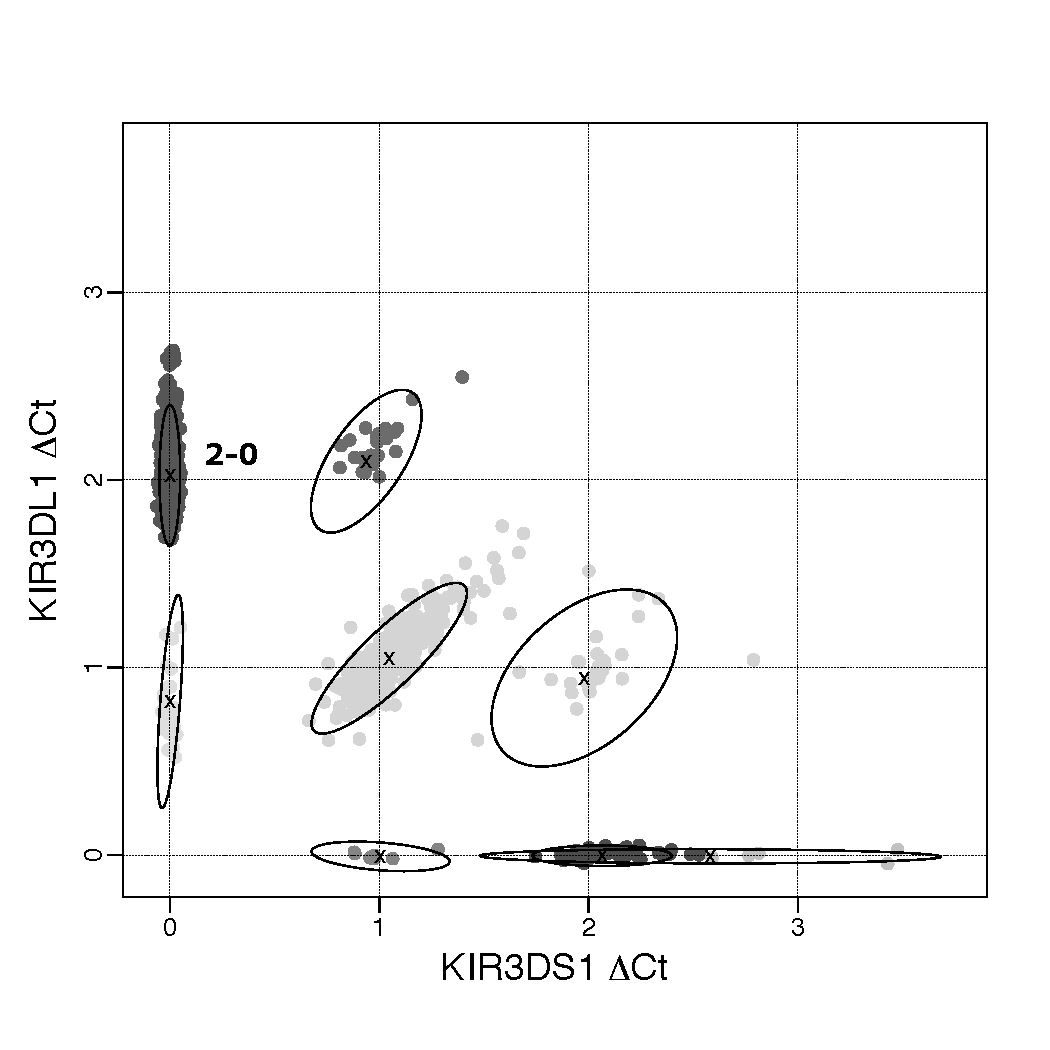
\includegraphics[scale=.5] {figures/genotyping-graytone.pdf}
        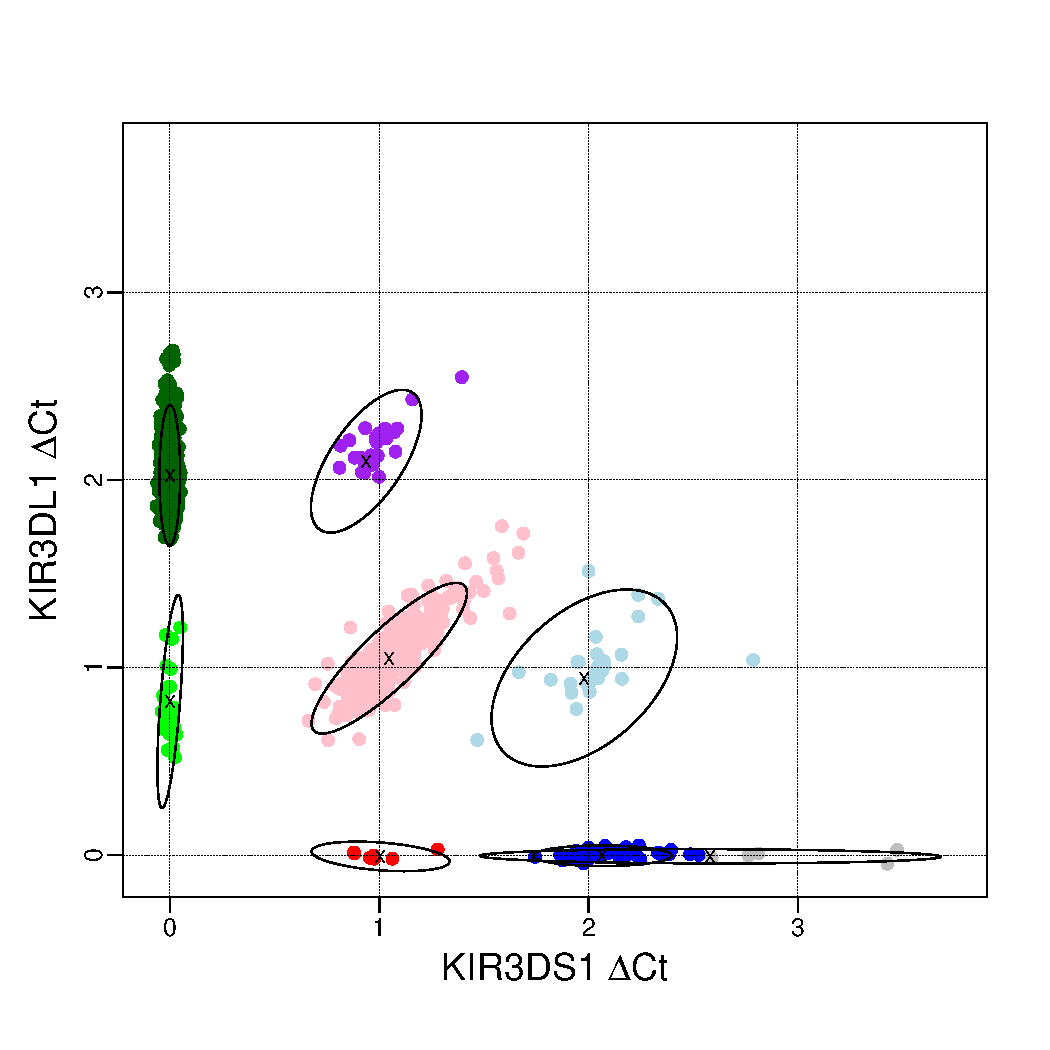
\includegraphics[scale=.5] {figures/genotyping.pdf}
    \end{subfigure}
    \begin{subfigure}[c]{.4\textwidth}\footnotesize
        %\texttt{
    \begin{tabular}{crrr}
      \toprule
      {\tiny KIR3DS1-KIR3DL1} & \multicolumn{3}{c}{count (percentage)} \\
          Copy Number & cases & controls & total \\ 
      \hline
        0-2 & 444 (59.44) & 446 (61.35) & 890 (60.38) \\ 
        1-1 & 229 (30.66) & 207 (28.47) & 436 (29.58) \\ 
        2-0 & 26 (3.48) & 28 (3.85) & 54 (3.66) \\ 
        2-1 & 15 (2.01) & 16 (2.2) & 31 (2.1) \\ 
        1-2 & 13 (1.74) & 14 (1.93) & 27 (1.83) \\ 
        0-1 & 13 (1.74) & 11 (1.51) & 24 (1.63) \\ 
        1-0 & 4 (0.54) & 3 (0.41) & 7 (0.47) \\ 
        3-0 & 3 (0.4) & 2 (0.28) & 5 (0.34) \\ 
      \midrule
      .-2 & 457 (61.18) & 460 (63.27) & 917 (62.21) \\ 
      .-1 & 257 (34.4) & 234 (32.19) & 491 (33.31) \\ 
      .-0 & 33 (4.42) & 33 (4.54) & 66 (4.48) \\ 
      \midrule
        0-. & 457 (61.18) & 457 (62.86) & 914 (62.01) \\ 
        1-. & 246 (32.93) & 224 (30.81) & 470 (31.89) \\ 
        2-. & 41 (5.49) & 44 (6.05) & 85 (5.77) \\ 
        3-. & 3 (0.4) & 2 (0.28) & 5 (0.34) \\ 
      \midrule
      Total &  747 (100) & 727 (100) & 1474 (100)\\ 
      \bottomrule
    \end{tabular}
    %}
    \end{subfigure}
    \caption{
        \label{figure:fuzzy-genotyping}
        On the left,
        the median normalised $\Delta$ct values for KIR3DS1 and KIR3DL1 are shown with
        the results of clustering into the eight genotype groups indicated by colouring points according to the group
        %the mixture of bivariate Gaussian clustering of the eight genotype groups.
        with the greatest posterior probability.
        The three most common genotype groups are the ones with normal copy numbers:
        KIR3DL1 homozygous (dark green), KIR3DL1/S1 heterozygous (pink) and KIR3DS1 homozygous (dark blue).
        %The rarer ones are: 2/1 (light blue), 1/2 (purple), 0/1 (light green), 1/0 (red) and 3/0 (gray).
        The ellipses delimit the $95^{th}$ percentile.
        On the right, the counts of the most probable bivariate genotypes are shown for cases and controls.
    }
\end{figure}



%\section{HLA typing}



\clearpage

%\section{T1D Association}


%\subsection{SNP}

\begin{table}[h]\footnotesize
%\begin{center}
    %\texttt{ %}
\begin{tabularx}{\textwidth}{ccrrrr|crrrr}
  \multicolumn{1}{l}{\bf{a)}} & \multicolumn{5}{c}{qPCR} & \multicolumn{5}{c}{SNP} \\
  \hline
    KIR3DS1/L1 & case:control & total & OR & 95\%CI & p-value & case:control & total  & OR & 95\%CI & p-value \\
  \hline
    0-2 & 444:446 &  890 & 1.00 &  &  & 4091:3220 &  7311  & 1.00 &  &  \\
    1-1 & 229:207 &  436 & 1.11 & 0.88-1.40 & 0.3673 & 2056:1628 &  3684  & 0.99 & 0.92-1.08 & 0.8828 \\
    2-0 & 26:28 &   54 & 0.92 & 0.52-1.61 & 0.7713 & 231:223 &   454  & 0.82 & 0.67-0.99 & 0.0349 \\
    2-1 & 15:16 &   31 & 0.94 & 0.46-1.93 & 0.8695 & 116:104 &   220  & 0.88 & 0.67-1.15 & 0.3422 \\
    1-2 & 13:14 &   27 & 0.93 & 0.43-2.01 & 0.8587 & 101:73 &   174  & 1.09 & 0.80-1.48 & 0.5833 \\
    0-1 & 13:11 &   24 & 1.19 & 0.53-2.68 & 0.6794 & 116:79 &   195  & 1.16 & 0.87-1.54 & 0.3273 \\
    1-0 & 4:3 &    7 & 1.34 & 0.30-6.02 & 0.7031 & 24:20 &    44  & 0.94 & 0.52-1.71 & 0.8509 \\
    3-0 & 3:2 &    5 & 1.52 & 0.27-8.62 & 0.6369 & 9:15 &    24  & 0.47 & 0.21-1.08 & 0.0756 \\
  \hline
    & 747:727 & 1474 &  &  &  & 6744:5362 & 12,106  &  & &  \\
  \\
  \multicolumn{1}{l}{\bf{b)}} & \multicolumn{5}{c}{qPCR} & \multicolumn{5}{c}{SNP} \\
  \hline
    KIR3DL1 & case:control & total & OR & 95\%CI & p-value & case:control & total  & OR & 95\%CI & p-value \\
  \hline
    .-2 & 457:460 &  917 & 1.00 &  &  & 4192:3293 &  7485  & 1.00 &  &  \\
    .-1 & 257:234 &  491 & 1.11 & 0.89-1.38 & 0.3702 & 2288:1811 &  4099  & 0.99 & 0.92-1.07 & 0.8464 \\
    .-0 & 33:33 &   66 & 1.01 & 0.61-1.66 & 0.9795 & 264:258 &   522  & 0.80 & 0.67-0.96 & 0.0159 \\
  \hline
    & 747:727 & 1474 &  &  &  & 6744:5362 & 12,106  &  & &  \\
  \\
  \multicolumn{1}{l}{\bf{c)}} & \multicolumn{5}{c}{qPCR} & \multicolumn{5}{c}{SNP} \\
  \hline
    KIR3DS1 & case:control & total & OR & 95\%CI & p-value & case:control & total  & OR & 95\%CI & p-value \\
  \hline
    0-. & 457:457 &  914 & 1.00 &  &  & 4207:3299 &  7506  & 1.00 &  &  \\
    1-. & 246:224 &  470 & 1.10 & 0.88-1.37 & 0.4096 & 2181:1721 &  3902  & 0.99 & 0.92-1.07 & 0.8750 \\
    2-. & 41:44 &   85 & 0.94 & 0.60-1.47 & 0.7787 & 347:327 &   674  & 0.83 & 0.71-0.97 & 0.0224 \\
    3-. & 3:2 &    5  & 1.24 & 0.21-7.28 & 0.8084 & 9:15 &    24  & 0.47 & 0.21-1.08 & 0.0741 \\
  \hline
    & 747:727 & 1474 &  &  &  & 6744:5362 & 12,106  &  & &  \\
\end{tabularx}
    \caption{
        \label{table:kir-t1d}
        No evidence of a significant joint or marginal effect of \emph{KIR3DS1/L1} copy number with T1D in qPCR dataset, 747 cases and 727 controls, and in SNP dataset, 6,744 cases and 5,362 controls.
    }
\end{table}


%\subsection{qPCR}


\begin{table}[h]\footnotesize
\begin{tabularx}{\textwidth}{ccrrrr|crrrr}
  \multicolumn{11}{c}{HLA-Bw4-80 subset} \\
  \multicolumn{1}{l}{\bf{a)}} & \multicolumn{5}{c}{qPCR} & \multicolumn{5}{c}{SNP} \\
  \hline
    KIR3DS1/L1 & case:control & total & OR & 95\%CI & p-value & case:control & total  & OR & 95\%CI & p-value \\
  \hline
    0-2 & 259:286 & 545 & 1.00 &  &  & 1025:1156 & 2181  & 1.00 &  &  \\
    1-1 & 123:128 & 251 & 1.06 & 0.79-1.43 & 0.6976 & 556:583 & 1139  & 1.08 & 0.93-1.24 & 0.3194 \\
    2-0 & 16:15 &  31 & 1.22 & 0.58-2.57 & 0.5985 & 61:87 &  148  & 0.79 & 0.56-1.11 & 0.1733 \\
    2-1 & 7:13 &  20 & 0.59 & 0.23-1.51 & 0.2754 & 32:40 &   72  & 0.90 & 0.56-1.45 & 0.6695 \\
    1-2 & 8:8 &  16 & 1.10 & 0.41-2.98 & 0.8450 & 27:32 &   59  & 0.95 & 0.57-1.60 & 0.8513 \\
    0-1 & 10:7 &  17 & 1.58 & 0.59-4.20 & 0.3621 & 36:26 &   62  & 1.56 & 0.94-2.60 & 0.0876 \\
    1-0 & 2:1 &   3 & 2.21 & 0.20-24.50 & 0.5187 & 7:3 &   10  & 2.63 & 0.68-10.19 & 0.1614 \\
    3-0 & 3:0 &   3 &  &  &  & 3:1 &    4  & 3.38 & 0.35-32.51 & 0.2910 \\
  \hline
    & 428:458 & 886 &  &  &  & 1747:1928 & 3,675  &  & &  \\
  \\

  \multicolumn{11}{c}{HLA-Bw4-80 subset} \\
  \multicolumn{1}{l}{\bf{b)}} & \multicolumn{5}{c}{qPCR} & \multicolumn{5}{c}{SNP} \\
  \hline
    KIR3DL1 & case:control & total & OR & 95\%CI & p-value & case:control & total  & OR & 95\%CI & p-value \\
  \hline
    .-2 & 267:294 & 561 & 1.00 &  &  & 1052:1188 & 2240  & 1.00 &  &  \\
    .-1 & 140:148 & 288 & 1.04 & 0.78-1.38 & 0.7787 & 624:649 & 1273  & 1.09 & 0.95-1.25 & 0.2414 \\
    .-0 & 21:16 &  37 & 1.45 & 0.74-2.83 & 0.2822 & 71:91 &  162  & 0.88 & 0.64-1.21 & 0.4399 \\
  \hline
    & 428:458 & 886 &  &  &  & 1747:1928 & 3,675  &  & &  \\
  \\
  \multicolumn{11}{c}{HLA-Bw4-80I subset} \\
  \multicolumn{1}{l}{\bf{c)}} & \multicolumn{5}{c}{qPCR} & \multicolumn{5}{c}{SNP} \\
  \hline
    KIR3DS1 & case:control & total & OR & 95\%CI & p-value & case:control & total  & OR & 95\%CI & p-value \\
  \hline
    0-. & 159:187 & 346 & 1.00 &  &  & 650:734 & 1384  & 1.00 &  &  \\
    1-. & 93:83 & 176 & 1.32 & 0.92-1.90 & 0.1370 & 384:365 &  749  & 1.19 & 0.99-1.42 & 0.0578 \\
    2-. & 12:14 &  26& 1.01 & 0.45-2.24 & 0.9842 & 61:75 &  136  & 0.92 & 0.64-1.31 & 0.6376 \\
    3-. & 2:0 &   2 &  &  &  & 1:0 &    1  & &  &  \\
  \hline
    & 266:284 & 550 &  &  &  & 1096:1174 & 2,270  &  &  &  \\
  \end{tabularx}
    \caption{
        \label{table:hla-bw4-kir-t1d}
        KIR3DS1/L1 association with T1D in the subset of individuals carriers of an HLA-Bw4 allele.
        KIR3DS1 association with T1D in the subset of individuals carriers of HLA-Bw4-80I alleles.
    }
\end{table}


%\section{Interaction with HLA-Bw4}



% latex table generated in R 3.0.0 by xtable 1.7-1 package
% Sat Aug 17 13:21:20 2013
\begin{table}[h]
\centering
%\vspace{1em}
\begin{tabularx}{\textwidth}{llrr|rr}
  \multicolumn{2}{l}{\bf{a)}} & \multicolumn{2}{c}{qPCR} & \multicolumn{2}{c}{SNP} \\
  \hline
  & & HLA-Bw4- & HLA-Bw4+ & HLA-Bw4- & HLA-Bw4+ \\ 
  \hline
  KIR3DS1- & KIR3DL1+ & 188 & 269 & 3146 & 1061 \\ 
  KIR3DS1+ & KIR3DL1- &  12 &  21 & 193 &  71 \\ 
  KIR3DS1+ & KIR3DL1+ & 119 & 138 & 1658 & 615 \\ 
  \hline
  & & $\chi^{2}_{2} = 2.3612$ & $p = 0.3071$ & $\chi^{2}_{2} = 2.7343$ & $p = 0.2548$ \\
  \\
  \multicolumn{2}{l}{\bf{b)}} & \multicolumn{2}{c}{qPCR} & \multicolumn{2}{c}{SNP} \\
  \hline
  & & HLA-Bw4- & HLA-Bw4+ & HLA-Bw4- & HLA-Bw4+ \\ 
  \hline
  \multicolumn{2}{c}{KIR3DL1-} &  12 &  21 & 193 &  71 \\
  \multicolumn{2}{c}{KIR3DL1+} & 307 & 407 & 4804 & 1676 \\
  \hline
  & & $\chi^{2}_{1} = 0.3286$ & $p = 0.5665$ & $\chi^{2}_{1} = 0.0916$ & $p = 0.7621$ \\
  \\
  \\
  \multicolumn{2}{l}{\bf{c)}} & \multicolumn{2}{c}{qPCR} & \multicolumn{2}{c}{SNP} \\
  \hline
  & & HLA-Bw4-80I- & HLA-Bw4-80I+ & HLA-Bw4-80I- & HLA-Bw4-80I+ \\ 
  \hline
  \multicolumn{2}{c}{KIR3DS1-} & 298 & 159 & 3557 & 650 \\ 
  \multicolumn{2}{c}{KIR3DS1+} & 183 & 107 & 2091 & 446 \\ 
  \hline
  & & $\chi^{2}_{1} = 0.257$ & $p = 0.6122$ & $\chi^{2}_{1} = 5.1171$ & $p = 0.02369$ \\
\end{tabularx}
%Pearson's Chi-squared test
%data:  table(kir, hlabw4)
%Pearson's Chi-squared test with Yates' continuity correction
%data:  table(kir3dl1, hlabw4)
\caption{
    \label{table:kir-hla}
    Case-only $\chi^{2}$ test in qPCR and SNP data.
    Distribution of KIR3DL1/S1 by relevant HLA-Bw4 genotype within cases.
    The test statistic and p value of chi-squared test is given for each contigency table.
    To reduce the degrees of freedom and improve power,
    we summarise copy numbers higher or equal than one by presence (+) and zero by absence (-).
    We find no significant association between KIR, for both compound and marginal genotypes, and HLA-Bw4 within cases.
}
\end{table}
%Pearson's Chi-squared test with Yates' continuity correction
%data:  table(kir3ds1, hlabw4I)




\FloatBarrier

\clearpage

%\section*{Tables}
%\input{tables}
\FloatBarrier



%\chapter{\label{flowsorting}{Flow Cytometry Cell Sorting}}
%\input{flowsorting}





\end{document}
